	% Set document type and scheme
	\documentclass[10pt]{beamer}
	\usetheme[progressbar=frametitle]{metropolis}

	% Load packages
	\usepackage{appendixnumberbeamer}
	\usepackage{booktabs}
	\usepackage[scale=2]{ccicons}
	\usepackage{pgfplots}
	\usepackage{xspace}
		\newcommand{\themename}{\textbf{\textsc{metropolis}}\xspace}
	\usepackage{stata}
	\usepackage{graphicx}
	\usepackage{lmodern}

	\title{Stata Workshop} %% that will be typeset on the
	\subtitle{} %% title page.
	\author{Roshni Khincha and Sakina Shibuya \\ DIME, World Bank}
	\date{August, 2018}

	\titlegraphic{%
		
\includegraphics[width=.2\textwidth]{DIME}\hfill % I think I should probably ask for a better image for this thing....
		
\includegraphics[width=.15\textwidth]{logo_minagri}\hfill
		
\includegraphics[width=.2\textwidth]{logo_eu}
		}

	\makeatletter
	\setbeamertemplate{title page}{
		\begin{minipage}[b][\paperheight]{\textwidth}
			\vfill%
			\ifx\inserttitle\@empty\else\usebeamertemplate*{title}\fi
			\ifx\insertsubtitle\@empty\else\usebeamertemplate*{subtitle}\fi
			\usebeamertemplate*{title separator}
			\ifx\beamer@shortauthor\@empty\else\usebeamertemplate*{author}\fi
			\ifx\insertdate\@empty\else\usebeamertemplate*{date}\fi
			\vfill
			\ifx\inserttitlegraphic\@empty\else\inserttitlegraphic\fi
			\vspace*{1cm}
		\end{minipage}
		}
	\makeatother

	\begin{document}
		
	\maketitle

	\section{Section 1: \\ Basics of Stata}

		% 1.1 Why learn stata?
		\begin{frame}
		
			\frametitle{\textsc{Why learn stata?}}
			\begin{center}
				\Large \textbf{Excel vs Stata} \\ \normalsize \text{Can I use Excel?}
			\end{center}
		
		\end{frame}

		
		\begin{frame}
			\frametitle{\textsc{The main reasons to use Stata}}
			\begin{itemize}
				\item In Excel you make changes directly to the data and save new versions of the data set
			
				\item In Stata you make changes to the instructions on how to get from the raw data to the final analysis and save new versions of the instructions
			
				\item Since Stata is a more statistics oriented software, processing the data to create analytical products can be a lot easier. 
			
			\end{itemize}
		\end{frame}



		\begin{frame}
			\frametitle{\textsc{The main reasons to use Stata}}
			\begin{itemize}
				\onslide<1-> \item Powerful tool with many capabilities:
				
				\begin{itemize}
					\item Descriptive statistics
					
					\item Inference statistics
					
					\item Complex data analysis
					
				\end{itemize}
				
				\onslide<2-> \item But it's also good for beginner programmers:
				
				\begin{itemize}
					\item User friendly interface
					
					\item Relatively easy programming language that can be learned while you're using the software
					
				\end{itemize}
			\end{itemize}
		\end{frame}	

		
	\begin{frame}
		\frametitle{\textsc{}}

		\begin{center}
			\Large \textbf{Stata interface}
		\end{center}
	\end{frame}
		
		
	\begin{frame}
		\frametitle{\textsc{The Stata interface}}
		
		\begin{figure}[H] 
		\centering
		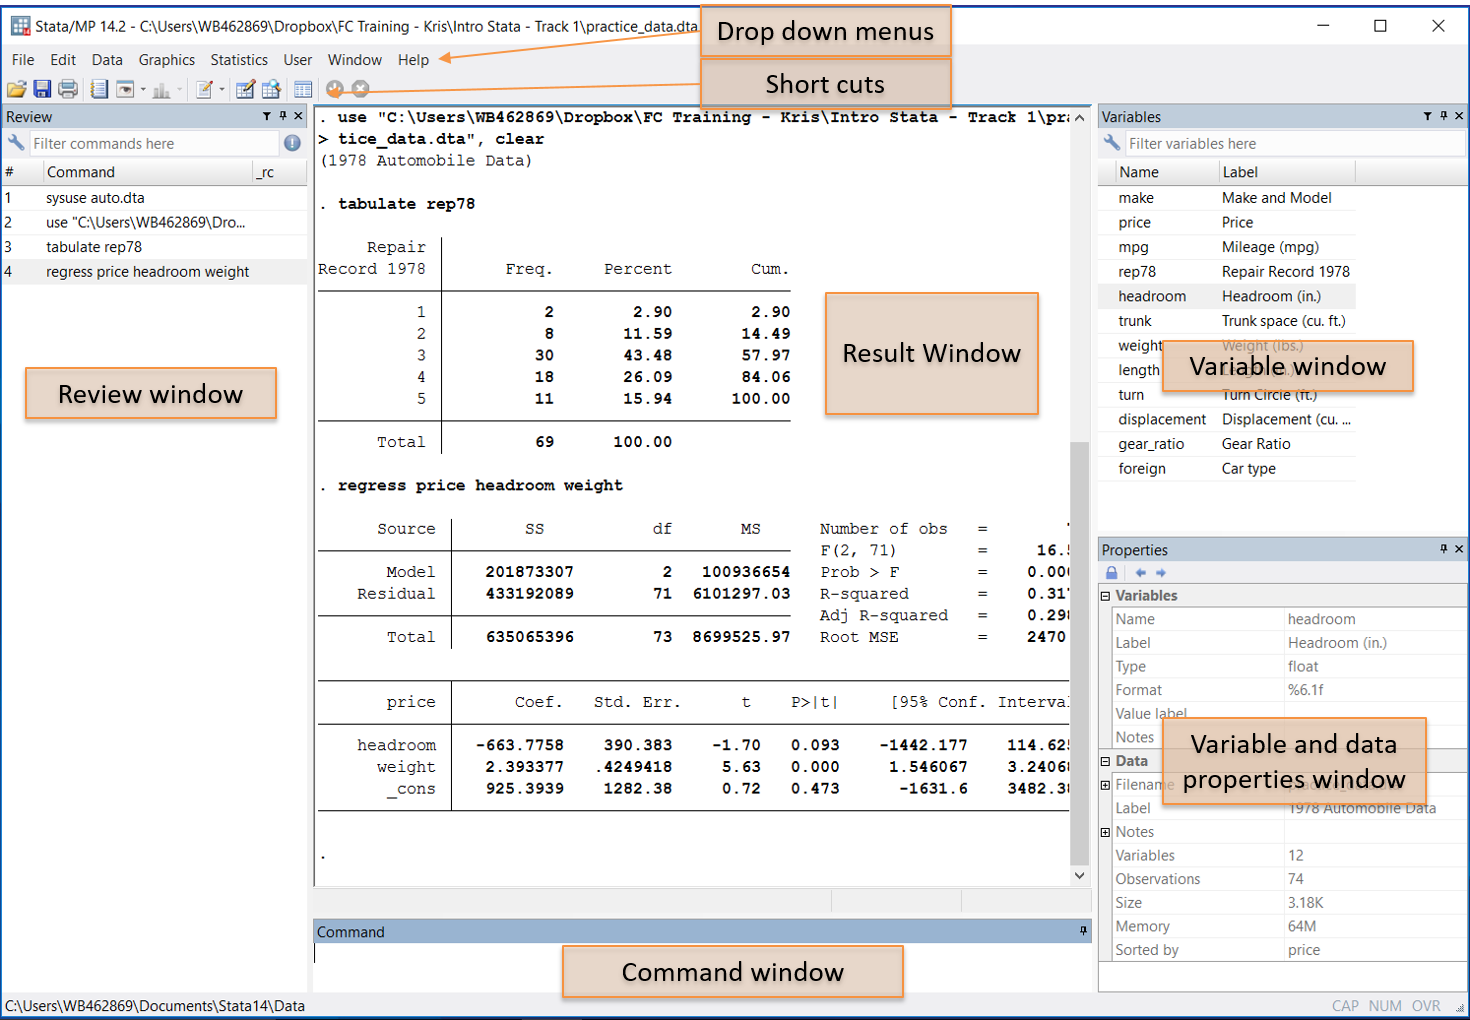
\includegraphics[width=0.9\linewidth]{stata_interface}
		\end{figure}
	\end{frame}

	\begin{frame}

		\frametitle{\textsc{The Stata interface - Review window}}
			\begin{center}
				\Large \textbf{} 
			\end{center}
		\begin{itemize}
			\item  Provides a history of your actions
			\item  A convenient way to bring back your previous commands and modify it to do something new
			\item Double click on a command you want to use again and it will appear in your command window
			\begin{itemize}
				\item You can also click in command window and select the commands in the result window by using \textit{PageUp/PageDown} buttons (or \textit{fn+ArrowUp/ fn+ArrowDown} on Mac)
			\end{itemize}
			\item If a command is \textcolor{red}{red} in the review window, it means it did not finish because an error
		\end{itemize}
	\end{frame}

	\begin{frame}
		\frametitle{\textsc{Filtering in variable and review windows}}
	\begin{minipage}{0.45\linewidth}
		\begin{itemize}
			\item  Both the variable and the review window will soon be very crowded. You can then search both of them for commands/variables
			
			\item  If you do not see the search bar, click the little funnel symbol
			
			
		\end{itemize}
	\end{minipage}
 	\hfill
	\begin{minipage}{0.45\linewidth}
		\begin{figure}[H] 
			\centering
			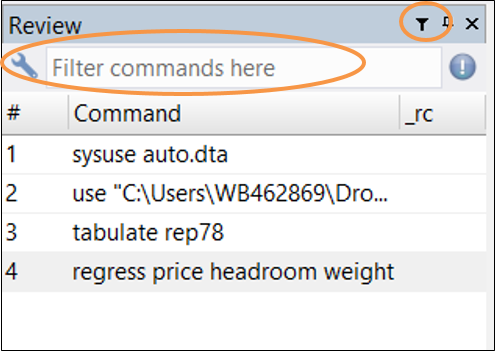
\includegraphics[width=0.75\linewidth]{review_window}
		\end{figure}
		\begin{figure}[H] 
			\centering
			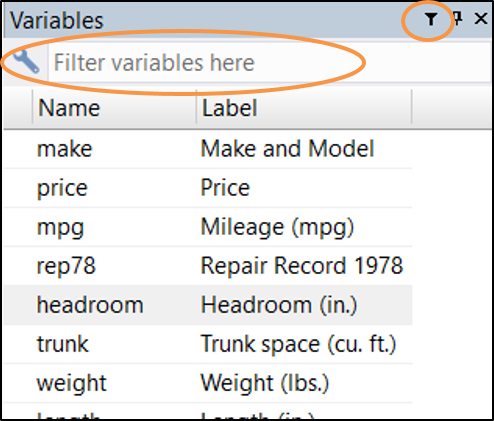
\includegraphics[width=0.75\linewidth]{variable_window}
		\end{figure}
	\end{minipage}
	\end{frame}


 
		\begin{frame}

			\frametitle{\textsc{}}
			\begin{center}
				\Large \textbf{How to open a data set in Stata} 
			\end{center}

		\end{frame}


		\begin{frame}
			\frametitle{\textsc{Three ways to tell stata what to do}}
			\begin{itemize}
				\onslide<1-> \item Drop-down menus
				
				\begin{itemize}
					\item An easy place to start but quickly becomes inefficient
					
				\end{itemize}
				
				\onslide<2-> \item Command window
				
			\begin{itemize}
				\item Faster than menus but require that you are familiar with the command
				
			\end{itemize}
				\onslide<3-> \item Do-file
				
			\begin{itemize}
				\item The only feasible way to run long instructions
				
				\item Use menus and command window to figure out what you need to write, then copy to a do file
				
			\end{itemize}
			\end{itemize}
		\end{frame}



		\begin{frame}
			\frametitle{\textsc{Open a dataset - menus}}
			 \begin{figure}[H] 
				\centering
				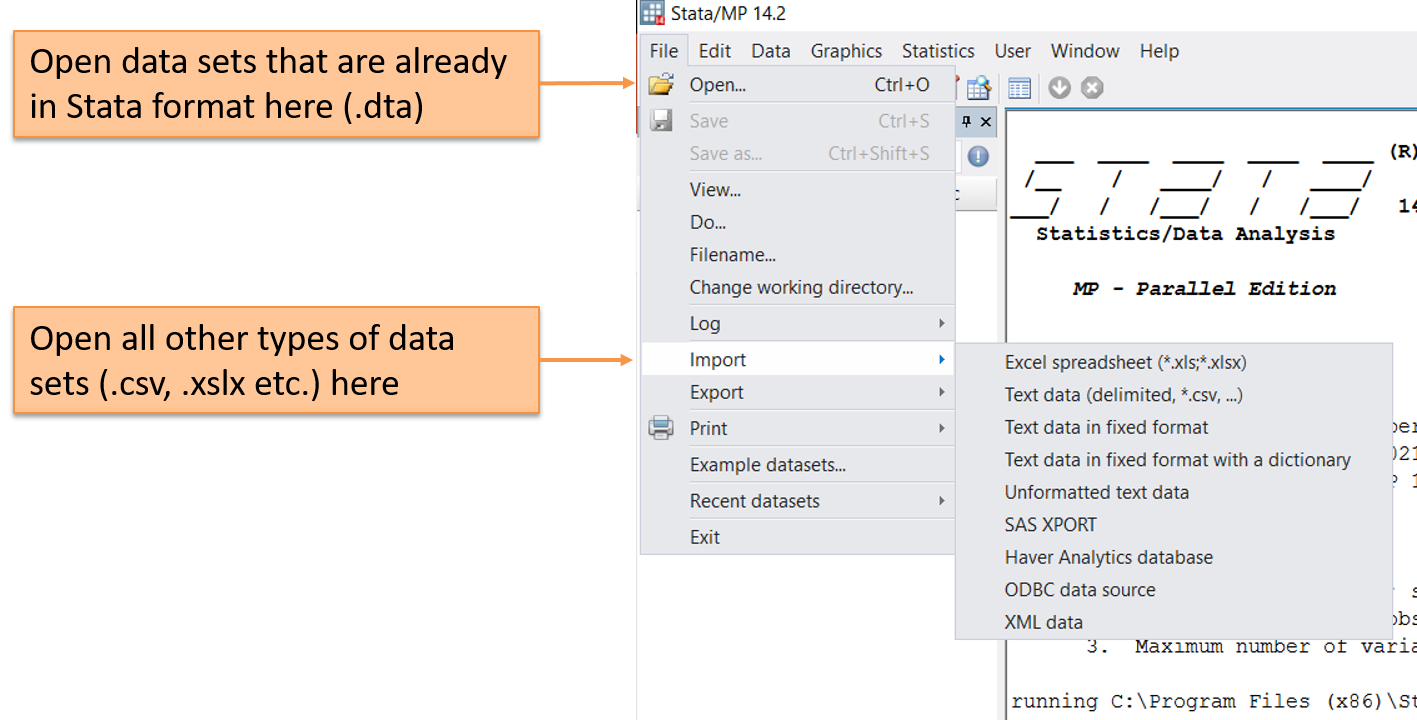
\includegraphics[width=0.9\linewidth]{open_dataset_menu}
			\end{figure}
		\end{frame}

	\begin{frame}
		\frametitle{\textsc{Open a dataset - command window}}
		\begin{figure}[H] 
			\centering
			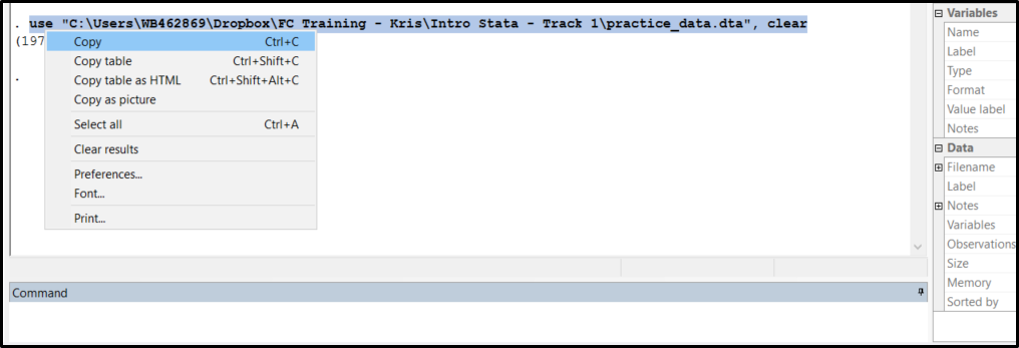
\includegraphics[width=0.9\linewidth]{open_dataset_command}
		\end{figure}
		\begin{itemize}
			\item When you use the menus, Stata produces the code for that action (except for Data Browse)
			\begin{itemize}
				\item Highlight, right-click and copy the code
				\item Paste the code in the command window
				\item Hit enter
			\end{itemize}
		\end{itemize}
	\end{frame}


	\begin{frame}
			\frametitle{\textsc{Task 1 - opening datasets}}
		\begin{enumerate}
			\onslide<1-> \item Open Stata and then open the EICV household data set \textbf{cs\_s0\_s5\_household.dta} using the menu: File $\rightarrow$ Open. Navigate to where you saved the material for this lab. Select the data set and click \textit{Open}
			\onslide<2-> \item Browse to check that you have data: Data  $\rightarrow$ Data Editor  $\rightarrow$ Data Editor Browse 
			\onslide<3-> \item Describe to get additional information on the data: Data  $\rightarrow$ Describe data $\rightarrow$ Describe data in memory or in a file.
			\begin{itemize}
				\item A new window will open
				\item Select In memory and press OK
			\end{itemize}
		\end{enumerate}
	\end{frame}

	\begin{frame}
			\frametitle{\textsc{Task 1 - opening datasets}}

		\begin{itemize}
			\item You can see that one the second command printed information on your screen.
			\begin{itemize}
				\item The first part is the command used
				\item The second part are the results
			\end{itemize}
		\end{itemize}

		 \begin{figure}[H] 
				\centering
				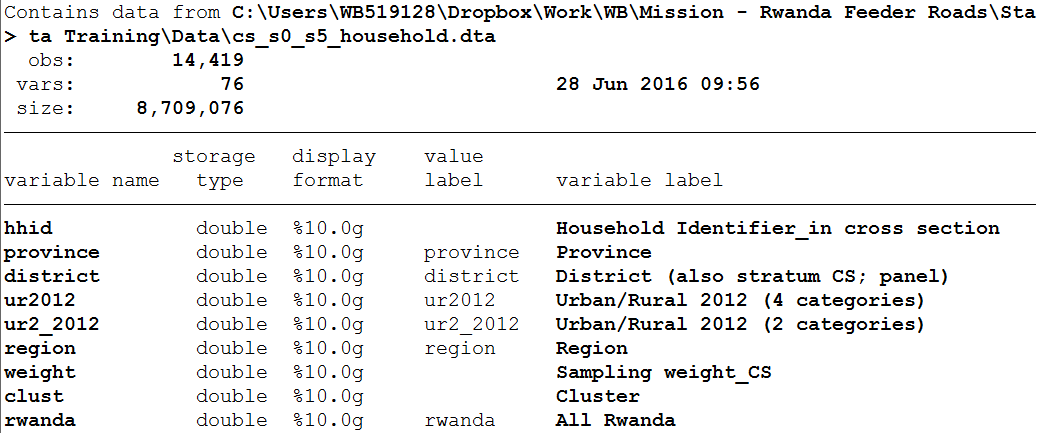
\includegraphics[width=0.9\linewidth]{task1}
		\end{figure}
	\end{frame}



	\begin{frame}
			\frametitle{\textsc{Task 1 - opening datasets}}
		\begin{itemize}
			\item You can perform both tasks by typing the in your command prompt. This will yield the same results
			
			\item Type \textit{browse} in the command window and press enter
			
			\item Type \textit{describe} and press enter
			
		\end{itemize}
	\end{frame}

	\begin{frame}
		\frametitle{\textsc{}}
		\begin{center}
			\Large  \textbf{Exploring a data set opened for the first time}
		\end{center}
	\end{frame}

	\begin{frame}
		\frametitle{\textsc{Exploring a new dataset}}
		\begin{itemize}
			\item To successfully clean a data set you must first understand the data set
			\item Some terminology:
			\begin{itemize}
				\item Columns are called variables
				\item Rows are called observations
			\end{itemize}
		\end{itemize}
	\end{frame}
		
		
	\begin{frame}
		\frametitle{\textsc{The EICV data}}
		\begin{itemize}
			\item For our exercises we will explore part of EICV 4 data
			\item The data is a household survey collected between 2013 and 2014 by NISR
			\item It is a cross-section of more than 14 thousand Rwandese households both in rural and urban areas
			\item Close to 2 thousand of these households form a panel have been also interviewed in EICV 3		
		\end{itemize}
	\end{frame}

	\begin{frame}
		\frametitle{\textsc{Types of variables}}
	
		\begin{itemize}
		\onslide<1->	\item 	In Stata, each variable (column) has to be either:
			\begin{itemize}
				\item string (text): values are red when browsing
				\item numeric (number): values are black or blue when browsing
			\end{itemize}
		\onslide<2->	\item Numbers \textbf{can} be stored as text, but text \textbf{cannot} be stored as number
			\begin{itemize}
				\item Not possible to do computations on numbers stored as text 		
			\end{itemize}
		\onslide<3->	\item Categorical variables should be stored as numeric variables and have labels
		\end{itemize}
	\end{frame}

	\begin{frame}
		\frametitle{\textsc{How the data looks}}	
		\begin{figure}[H] 
			\centering
			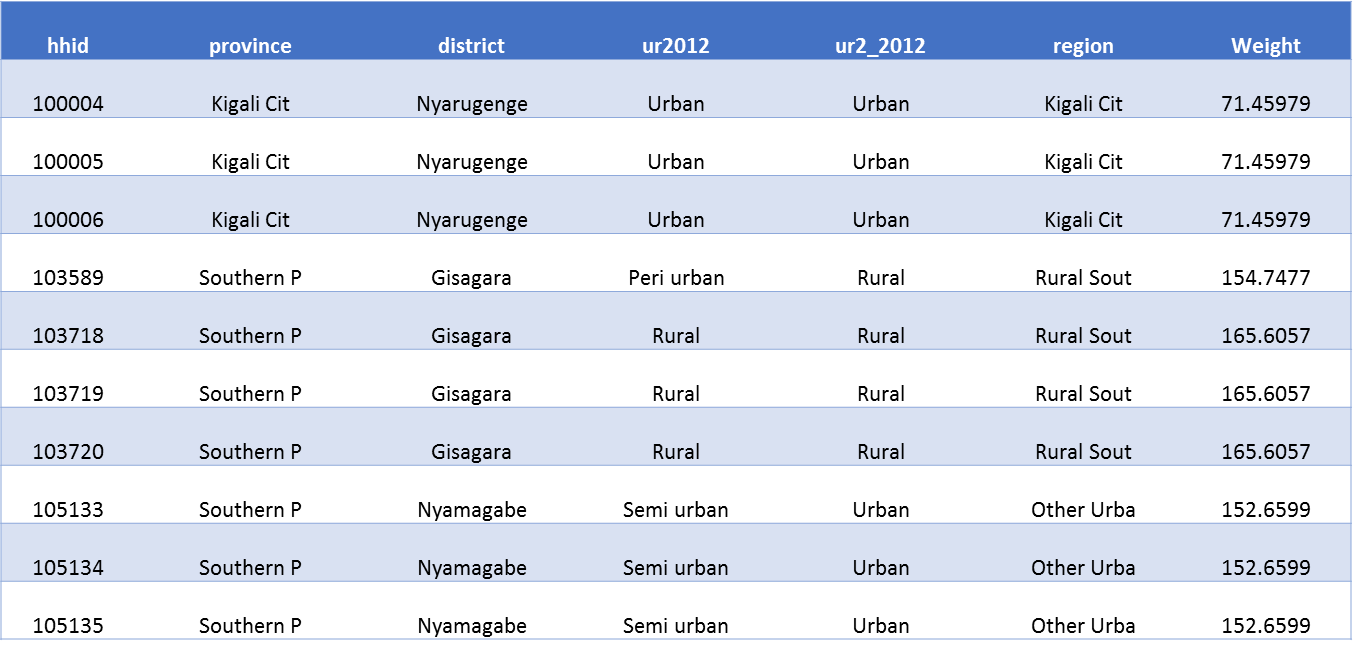
\includegraphics[width=0.9\linewidth]{dataset1}
		\end{figure}
	\end{frame}
	\begin{frame}
		\frametitle{\textsc{How the data actually is}}	
		\begin{figure}[H] 
			\centering
			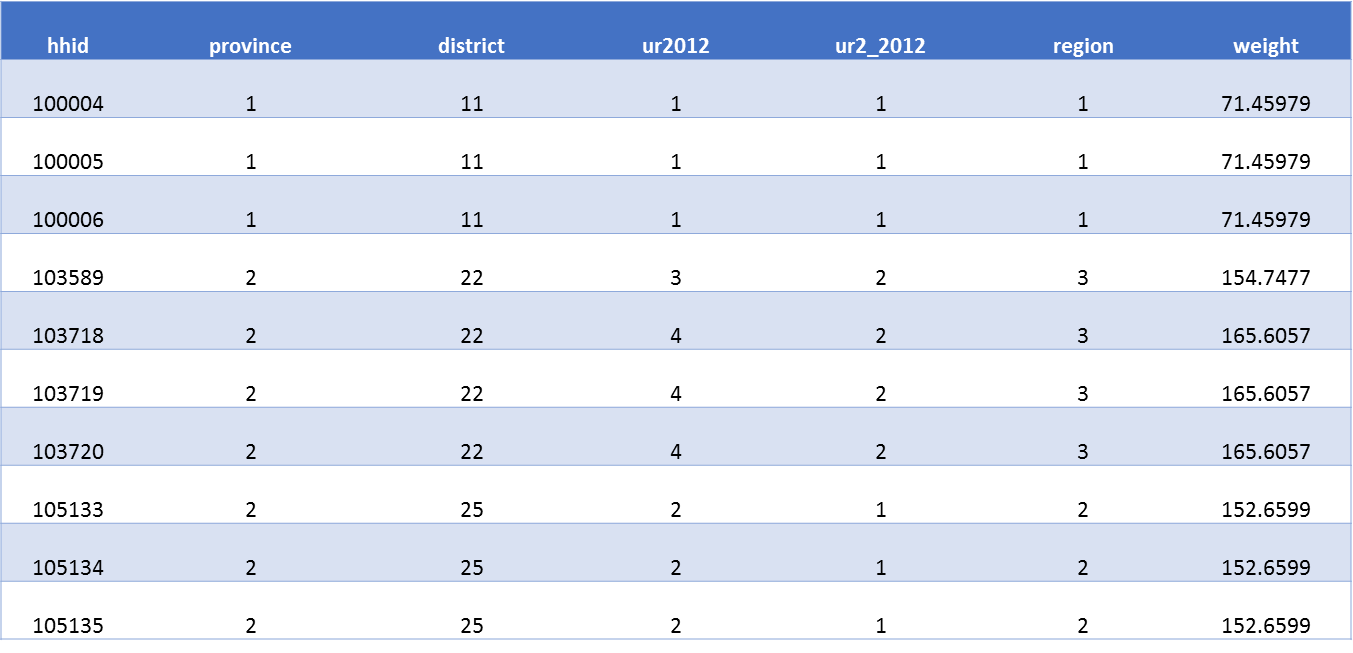
\includegraphics[width=0.9\linewidth]{dataset2}
	\end{figure}	
	\end{frame}


	\begin{frame}
		\frametitle{\textsc{Useful commands}}

		\begin{itemize}
		\onslide<1->	\item 	\textit{\underline{br}owse}: see all data in spreadsheet format
		\onslide<1->	\item \textit{\underline{d}escribe}: list of all variables in memory
			\begin{itemize}
				\item Total number of variables \& observations (size of matrix)
				\item Variable name, type, format, value label name, variable label
			\end{itemize}
		\onslide<1->	\item \textit{\underline{su}mmarize}: Basic statistics for numeric variables
			\begin{itemize}
				\item Obs (Number of observations), Mean, Std. Dev. (Standard deviation), Min (Minimum), Max (Maximum)
			\end{itemize}
		\onslide<1->	\item \textit{\underline{tab}ulate}: frequencies
			
		\end{itemize}
	\end{frame}

	\begin{frame}
		\frametitle{\textsc{More commands}}
		\begin{itemize}
			\onslide<1->\item 	\textit{codebook}: displays the following for each variable
		
			\begin{itemize}
				\item Type (more detail than describe)
				\item Number of unique values and number of missing values
				\item Range and units
				\item Examples of values (strings); tabulations (categorical); or mean, sd and percentiles (continuous)
				\item Warnings if embedded blanks (may or may not be ok)
			\end{itemize}
			\onslide<2->\item \textit{labelbook}: displays the following for each stored value label
			\begin{itemize}
				\item Label definitions
				\item Which variables labels are applied to
			\end{itemize}
			\onslide<3->\item \textit{\underline{l}ist}: lists all variables and observations
			\begin{itemize}
				\item Can qualify: \textit{list if price \textless 5000, list in 1/10}
			\end{itemize}
			\onslide<4->\item \textit{\underline{su}mmarize, \underline{d}etail} : percentiles, variance, skewness, kurtosis
			
		\end{itemize}
	\end{frame}

	\begin{frame}
		\frametitle{\textsc{Task 2 - exploring a data set}}
		\begin{enumerate}
			\onslide<1-> \item Open the \textbf{cs\_s0\_s5\_household.dta} again. Use the command prompt this time.
			\onslide<2-> \item Explore the dataset
			\begin{itemize}
				\item browse - see the different colors in the columns
				\item describe - check the storage type column
				\item summarize - are there any statistics that might not make sense to interpret?
			\end{itemize}
			\onslide<3->\item Learn more about the variable \textit{s5bq3a}, the household estimated rent amount. What values does it take on? What is minimum, maximum, mean of this variable? How many unique values does it have?
		\end{enumerate}
		
\begin{stlog}tabulate s5bq3a
summarize s5bq3a 
codebook s5bq3a
\end{stlog}
		\end{frame}

	\begin{frame}
		\frametitle{\textsc{Task 2 - exploring a data set}}

	\onslide<1->	\begin{itemize}
			\item Learn more about the variable \textit{ur2012}, to learn about the proportion of urban and rural households in Rwanda
	
			
\begin{stlog}. tabulate ur2012 
\end{stlog}
		\begin{itemize}
				\item Now Create a pie chart: Graphics $\rightarrow$ Pie chart, select \textit{ur2012} as Category variable and press OK
			\end{itemize}
		\onslide<2-> \item Now, create a pie-chart graph for the variable \textit{s5cq7}, the type drinking water source used. This time, use the command prompt!
			\begin{itemize}
				\item Use the code printed by the previous graph and replace the name of the variable
			\end{itemize}

		\end{itemize}
	\end{frame}

	\begin{frame}
		\frametitle{\textsc{Tips and resources}}
		\begin{itemize}
			\item Using help - Type \textbf{\textit{help summarize}} to get documentation on the summarize function
			\item Using search - Type \textbf{\textit{search regression}} to get general documentation on running regressions in Stata
			\item Google - Search what you want to do. There are many resources online (e.g. Statalist)
			
		\end{itemize}
	\end{frame}
			 
\section{Section 2: \\ Editing data}

	\begin{frame}
		\frametitle{\textsc{}}

		\begin{center}
			\Large \textbf{Editing data in Stata}
		\end{center}
	\end{frame}

	\begin{frame}
		\frametitle{\textsc{Deleting variables}}

		\begin{itemize}
			\item You can delete variables using the commands \textbf{\textit{drop}} 
				  or \textbf{\textit{keep}}
			\item Deleting variables is useful to
			\begin{itemize}
				\item Simplify a very complex data-set for you to work with	
				\item Reduce computational time when dealing with large data-sets
				\item Create temporary subsets of data for analytical purposes, like creating a table or graph
			\end{itemize}
			\item WARNING: be careful not save the new data on top of the original
		\end{itemize}
	\end{frame}

	\begin{frame}
		\frametitle{\textsc{Task 3 - deleting variables}}

		\begin{itemize}
		\onslide<1->	\item Open the \textbf{cs\_s0\_s5\_household.dta} data set (use the command prompt)
		\end{itemize}
	
		\begin{itemize}
		\onslide<2->	\item Keep the variables we will use in this excerise by typing
		\end{itemize}
	
\begin{stlog}. use "$data\\cs_s0_s5_household.dta", clear
{\smallskip}
\end{stlog}
		\begin{itemize}
		\onslide<3->	\item Now let's say we kept a few variables that we didn't actually needed.To drop them, type
		\end{itemize}
	
\begin{stlog}. keep hhid province district ur2012 s5cq2 s5cq4 s5cq8 s5cq15 s5cq23 s5bq2 s5cq22 s5cq1
> 3 s5cq17 
{\smallskip}
\end{stlog}
	\end{frame}
	
	\begin{frame}
		\frametitle{\textsc{Renaming variables}}
		\begin{itemize}
			\item You can use the command \textbf{\textit{rename}} to change the names of your variables
			\item Renaming is useful as
			\begin{itemize}
				\item Can make your life easier when programming. Especially when the original variable names don't make much sense
				\item It helps you remember what the variable means when a meaningful name is chosen
				\item Picking a short variable name reduces time when typing it
				
			\end{itemize}
		\end{itemize}
	\end{frame}
			
	\begin{frame}
		\frametitle{\textsc{Task 4 - renaming variables}}
		\begin{itemize} 
			\item Rename all the remaining variables. Type the code below, one line at a time
		\end{itemize}
\begin{stlog}. drop province s5bq2 s5cq17 s5cq15
{\smallskip}
\end{stlog}
	\end{frame}
	
	\begin{frame}
		\frametitle{\textsc{Generating variables}}
		\begin{itemize}
			\item You can use the command \textbf{\textit{\underline{gen}erate}} to create new variables		
			\item Generating variables can be useful to
			\begin{itemize}
				\item Change the values of a variable to a different measurement unit
				\item Create a dummy variable identifying if how many observations have a given characteristic
			\end{itemize}
		\end{itemize}		
	\end{frame}		
	
	
	\begin{frame}
		\frametitle{\textsc{Task 5 - generating variables}}
		\begin{itemize} 
			\item Let us create a variable that converts the number of meters to the main water source to centimeters. Type:
		\end{itemize}
\begin{stlog}generate  cm_main_ws = m_main_ws*100
\end{stlog}
		\begin{itemize}
			\item Now get descriptives for the new variable using \textit{summarize}
		\end{itemize}
	\end{frame}
	
	
	\begin{frame}
		\frametitle{\textsc{Task 5 - generating variables}}
		\onslide<1->\begin{itemize} 
			\item Let us create a dummy variable (that assumes values 0 or 1) to see if the main water source is the same as the used water source. 
		\onslide<2->	\item First create a variable that equals zero
		\end{itemize}
\begin{stlog}. generate  cm_main_ws = m_main_ws*100
(1,098 missing values generated)
{\smallskip}
\end{stlog}
		\begin{itemize}
		\onslide<3->	\item Now let's replace that with 1 when it satisfies the condition that the two variables are equal. Type:
		\end{itemize}
\begin{stlog}. gen  d_closest_ws        = 0
{\smallskip}
\end{stlog}
		\begin{itemize}
		\onslide<4->	\item Finally, tabulate the data using the function \textit{tabulate}
		\end{itemize}		
	\end{frame}
	
	\begin{frame}
		\frametitle{\textsc{Labeling variables and values}}
		\begin{itemize}	
			\item Labeling variables helps understand the variable 
			\item Value labels indicate what each category of a categorical variable stands for
			\item Labeling variables and values is essential for easier understanding in the future by you and others
		\end{itemize}
	\end{frame}
		
	\begin{frame}
		\frametitle{\textsc{Task 6 - labeling}}
		\begin{itemize}
			\item Let us create a label for the two variables we created in Task 5
		\end{itemize}
\begin{stlog}. replace d_closest_ws = 1 if m_main_ws == m_used_ws
(10,250 real changes made)
{\smallskip}
\end{stlog}
	
		\begin{itemize}
			\item Check the variable window to see the label!
		\end{itemize}		
	\end{frame}	
	

	\begin{frame}
		\frametitle{\textsc{Task 6 - labeling}}
		\begin{itemize}
		\onslide<1-> 	\item We can also create labels for values with the functions \textit{label define} and \textit{label values}. Type:
		\end{itemize}
\begin{stlog}label define yes_no_lb 1 "Yes" 0 "No"
label values d_closest_ws yes_no_lb
\end{stlog}
	
		\begin{itemize}
	\onslide<2-> 		\item You can see the labels if you tabulate the labeled variable or browse the data
			\item This is very useful for binary or categorical variables when visualizing the data
		\end{itemize}		
	\end{frame}		
	
	
	\begin{frame}
		\frametitle{\textsc{Refresher}}
		On day 1 we learnt ...
		\begin{itemize}
			\item how stata works
			\item using the dropdown and command window to execute actions
			\item how to explore a dataset using commands like \textit{browse describe tabulate summarize}
			\item how to manipulate a dataset using commands like \textit{drop keep generate replace}
			\item how to label variables and values
		\end{itemize}
	\end{frame}
	
	\begin{frame}
		\frametitle{\textsc{}}

		\begin{center}
			\Large  \textbf{How to share your work with your team}
		\end{center}
	\end{frame}

	\begin{frame}
		\frametitle{\textsc{You are asked to share your work}}

		\begin{itemize}
			\item How would you share the work you have done so far?
			\item Send only the data set? That would be like Excel and only shares the latest version of the data
			\item Nowadays there's a greater demand than to share more than the latest version of the data. We need to show what we did
			\item This is where .do files come into the picture

		\end{itemize}
	\end{frame}

		\begin{frame}
			\frametitle{\textsc{What's the fuss about do-files?}}
			
			\begin{itemize}
				\item It's through the do-file you communicate your work to other members in your team, both current and future
				\item Think of the do-files as instructions on how to get from raw data to final report
				\item For a simple task you can enter commands manually. But for more complex tasks you need to write a recipe, or a list of instructions
				\item A do-file works similarly to the command window. But instead of running one line of code at the time, a do-file lets you do that run any number of lines of code

				
				\end{itemize}
			\end{frame}
			
	\begin{frame}
		\frametitle{\textsc{Do-files}}
		\begin{itemize}
			\item Open up a new do-file. Window $\rightarrow$ Do-file Editor $\rightarrow$ New Do-file Editor
			\item Alternatively click the shortcut highlighted below:
		\end{itemize}
		\begin{figure}[H] 
			\centering
			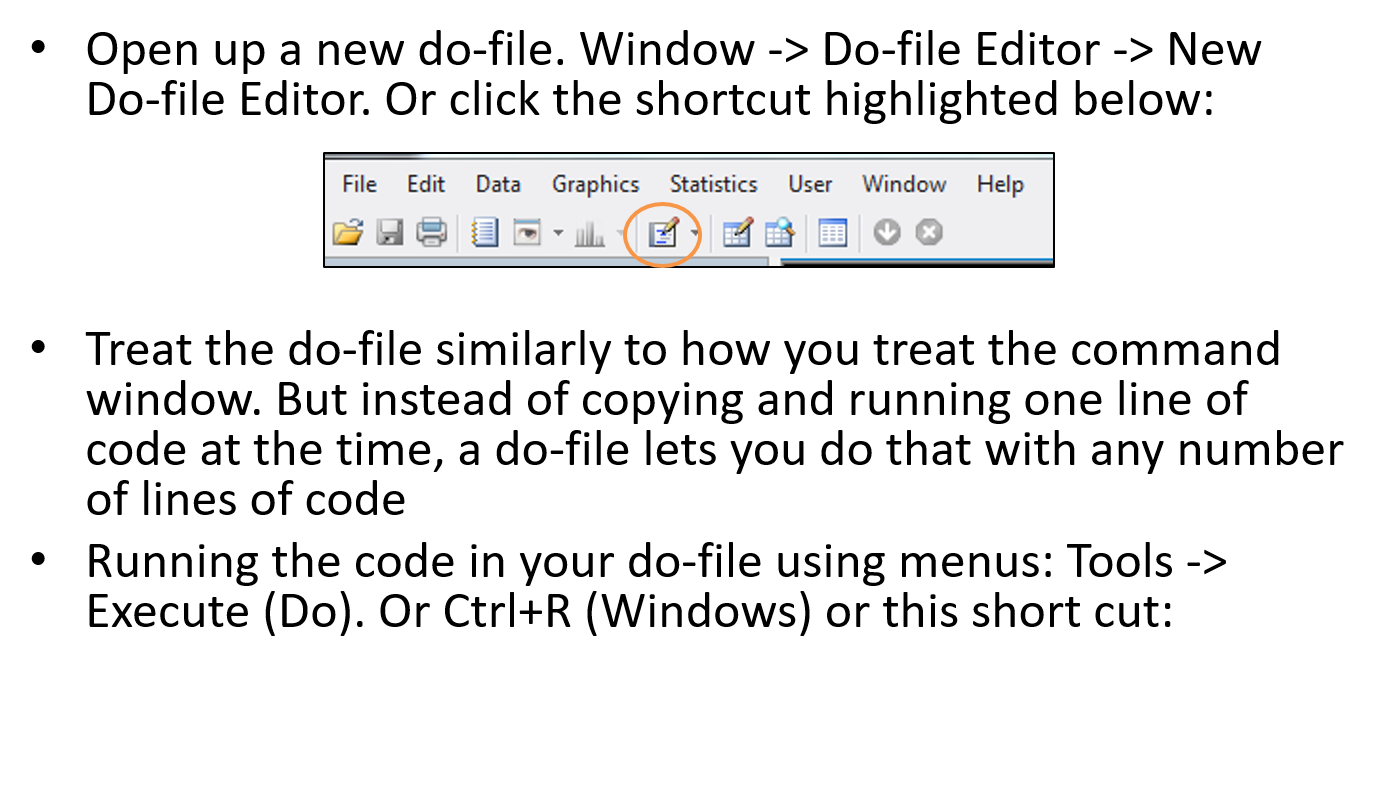
\includegraphics[width=0.9\linewidth]{dofile}
		\end{figure}
	\end{frame}
	\begin{frame}
		\begin{itemize}
			\item Running the code in your do-file using menus: Tools $\rightarrow$ Execute (Do) 
			\item Alternatively, select Ctrl+D (Windows) on your keyboard
			\item Alternatively, click the shortcut highlighted below
		\end{itemize}
		\begin{figure}[H] 
			\centering
			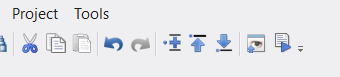
\includegraphics[width=0.9\linewidth]{run}
		\end{figure}		
		
	\end{frame}
	
	\begin{frame}
		\frametitle{\textsc{How do you find a file path?}}		
		\begin{itemize}
			\item File path are a integral part of sharing data which we will explain in the next slide
		\end{itemize}
		\begin{figure}[H]
			\centering
			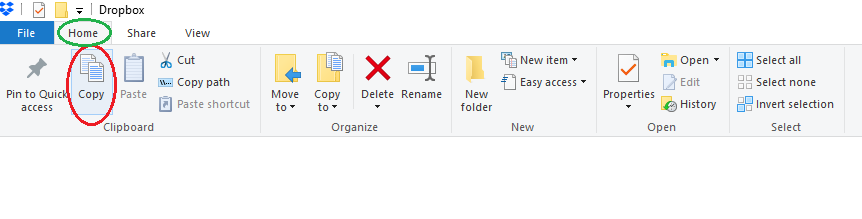
\includegraphics[width=0.9\linewidth]{file_path}
		\end{figure}
		\begin{itemize}
			\item When you open any folder, clicking on the \textbf{Home} button on the top right
			\item Then clicking on \textbf{Copy} copies the path to the folder you opened
		\end{itemize}
	\end{frame}
	
	\begin{frame}
	\frametitle{\textsc{Macros}}

		\begin{itemize}
			\item You need to be at least familiar with this topic as this technique is critical especially when projects grow in size
			\item Macros (globals, locals, scalar) save some information 
				 (text or number) that you can reference later
				\begin{itemize}
					\item Example: We want to access files in the folder 
								   multiple times. We can store the folder 
								   location in a global and use it multiple times
				\end{itemize}
			\item To call a global saved we use the \$ symbol
		\end{itemize}
	\end{frame}	
	
	\begin{frame}
		\frametitle{\textsc{Task 7 - using a do-file}}
		\begin{itemize}
			\item Open a new do-file. Save it! 

			\item Type the following in your do file
			\end{itemize}
\begin{stlog}clear all
\end{stlog}
		\begin{itemize}
			\item Open the folder where you saved the data we shared
			\item Copy the file path of this folder
			\item Create a \textbf{global} called \textit{data} using the file path you copied
		\end{itemize}
\begin{stlog}. global  data "$dropbox\\minagri_stata_training_aug2018\\data"
{\smallskip}
\end{stlog}
	\end{frame}
		
	\begin{frame}
		\frametitle{\textsc{Task 7 - using a do-file}}
		
		
	\begin{itemize}
			\item Next, use the review window to copy to your do-file all the actions you already did:
			\begin{itemize}
				\item Now run the do-file
				\item Load the dataset using the global you created
				\item Keep only the variables that you need
				\item Drop the ones you forgot
				\item Rename all the variables
				\item Create the cm to the main water source variable
				\item Create the dummy if main water source is the same as the used water source
				\item Label the variables and values
			\end{itemize}
		\end{itemize}	
	\end{frame}
		
	\begin{frame}
		\frametitle{\textsc{Task 7 - using a do-file}}
		This is how your do-file should look now
\begin{stlog}. quietly use "$data\\cs_s0_s5_household.dta", clear 
{\smallskip}
. quietly rename s5cq2 m_main_ws
{\smallskip}
. gen  cm_main_ws = m_main_ws*1000
(1,098 missing values generated)
{\smallskip}
\end{stlog}
	\end{frame}

	\begin{frame}
		\frametitle{\textsc{Task 7 - editing a do-file}}
	
		\begin{itemize}
			\item Now let's edit the do-file!
			\item We just realized that the number of centimeters to the main water source doesn't make much sense. Let's edit it to the number of kilometers. Replace the code:
			\end{itemize}
\begin{stlog}. quietly use "$data\\cs_s0_s5_household.dta", clear
>  
{\smallskip}
. quietly rename s5cq2 m_main_ws
{\smallskip}
. gen  km_main_ws = m_main_ws/1000
(1,098 missing values generated)
{\smallskip}
\end{stlog}
	to
\begin{stlog}use "$data\\cs_s0_s5_household.dta", clear
\end{stlog}
	Also, remember to edit the label before you run the do-file!
	\end{frame}
	
	\begin{frame}
		\frametitle{\textsc{Comments}}	
		\begin{itemize}	
			\item Comments is the green text you have seen in the code examples
			\item Comments is text that Stata will ignore when running your code
			\item Comments is what makes the difference between instructions that are easy to follow or impossible to understand
			\item You can also use comments to omit certain parts of your do-file that you don't want to run anymore, but don't want to erase
			\begin{itemize}
				\item Maybe you might need it in the future! Just be careful, keeping lots of old code in your do-file might make it messy and hard to understand.
			\end{itemize}
		\end{itemize}
	\end{frame}
	
	\begin{frame}
		\frametitle{\textsc{Different types of comments}}
		\begin{center}	
			\Large\textbf{}
		\end{center}	
		\begin{enumerate}	
			\onslide<1-> \item \textit{/* comment */} 
			\begin{itemize}
				\item Used for long comments or to explain many lines of code in the following section
			\end{itemize}
			\onslide<2-> \item \textit{* comment} 
			\begin{itemize}
				\item Used to explain what happens on the following few rows
			\end{itemize}
			\onslide<3-> \item \textit{ // comment} 
			\begin{itemize}
				\item Used to explain the same line of code
			\end{itemize}
		\end{enumerate}
	\end{frame}
	
	
	\begin{frame}
		\frametitle{\textsc{Task 8 - commenting}}

		\begin{itemize}	
			\item Now that you know about comments, add them to your do-file! 
			\onslide<1-> \item First, add a title and a brief explanation of what your do-file does (e.g. Stata training do-file : Uses EICV4 data to practice Stata, limiting the variables to water usage)
			\onslide<2-> \item Now, add a heading to every main section of your do-file (e.g. load data, keep the variables I'll use, create new variables, etc.)
			\onslide<3-> \item Finally, we realized that we actually don't need the \textit{km\_main\_ws}  variable now, but don't want to erase the code because we might want to use it in the future. Comment out that variable's creation.
			\item Run everything!
		\end{itemize}

	\end{frame}
	
		
	\begin{frame}
		\frametitle{\textsc{Task 8 - commenting}}

		\begin{itemize}	
			\item Did it work? 

			\item If you comment out the variable creation and not the labeling, you probably got an error like this:
		\end{itemize}
		\begin{figure}[H] 
			\centering
			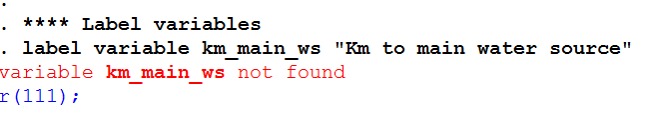
\includegraphics[width=0.9\linewidth]{error}
		\end{figure}
		\begin{itemize}
			\item To avoid this, comment out the labeling of the \textit{km\_main\_ws} variable as well. 
		\end{itemize}

	\end{frame}
			
	\begin{frame}
	\frametitle{\textsc{Saving Stata datasets}}	
		\begin{itemize}
			\item The command for saving a Stata dataset is \textit{\textbf{save}}.
			\item \textit{save} saves your data in memory in a file format called dta. 
				  This is a file that can only be read with Stata.
			\item The command for saving a dataset in excel and csv is \textit{\textbf{export}}.
			\item \textit{\textbf{export}} is the opposite of import, and is very versatile. 
				  It lets you save data in excel, csv, sas and others. 
				  Please refer to the help file on \textit{\textbf{export}}.
		\end{itemize}	
	\end{frame}

	\begin{frame}
	\frametitle{\textsc{Saving Stata datasets}}	
		\begin{columns}
			\begin{column}{0.5\textwidth}
				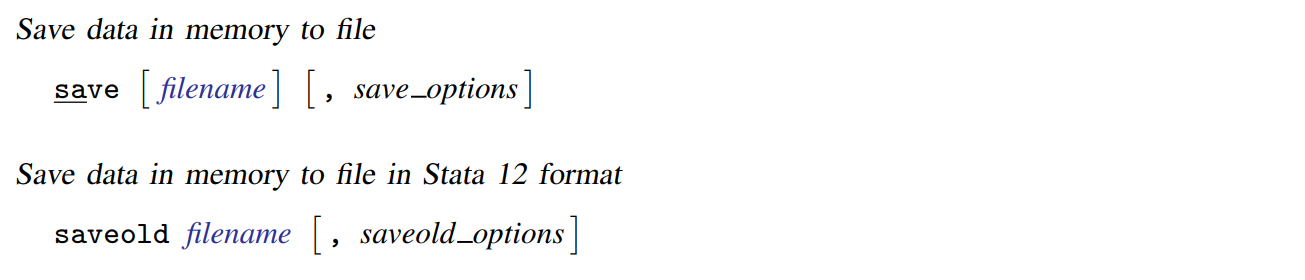
\includegraphics[width=\linewidth]{helpfile_save_1}
				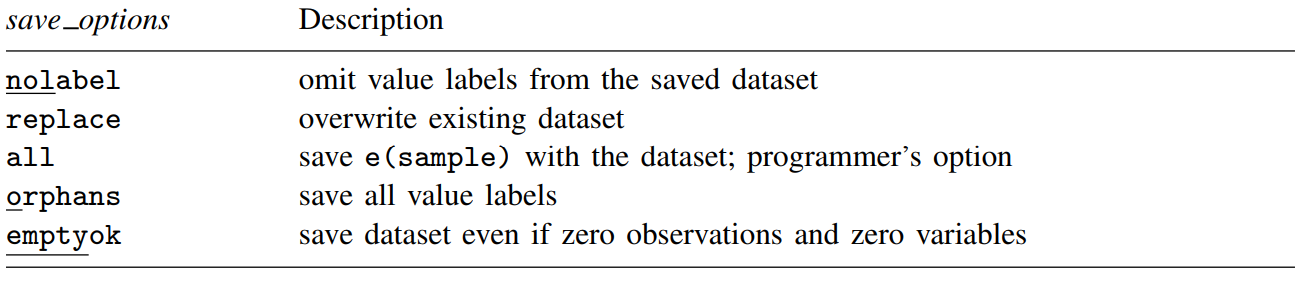
\includegraphics[width=\linewidth]{helpfile_save_2}
			\end{column}
			\begin{column}{0.5\textwidth}
				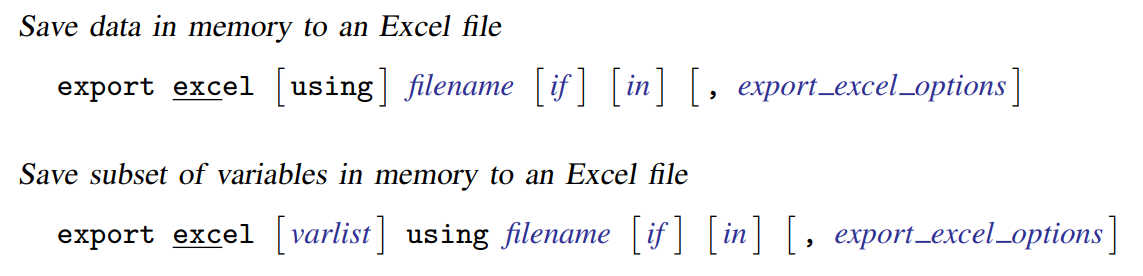
\includegraphics[width=\linewidth]{helpfile_exportexcel_1}
				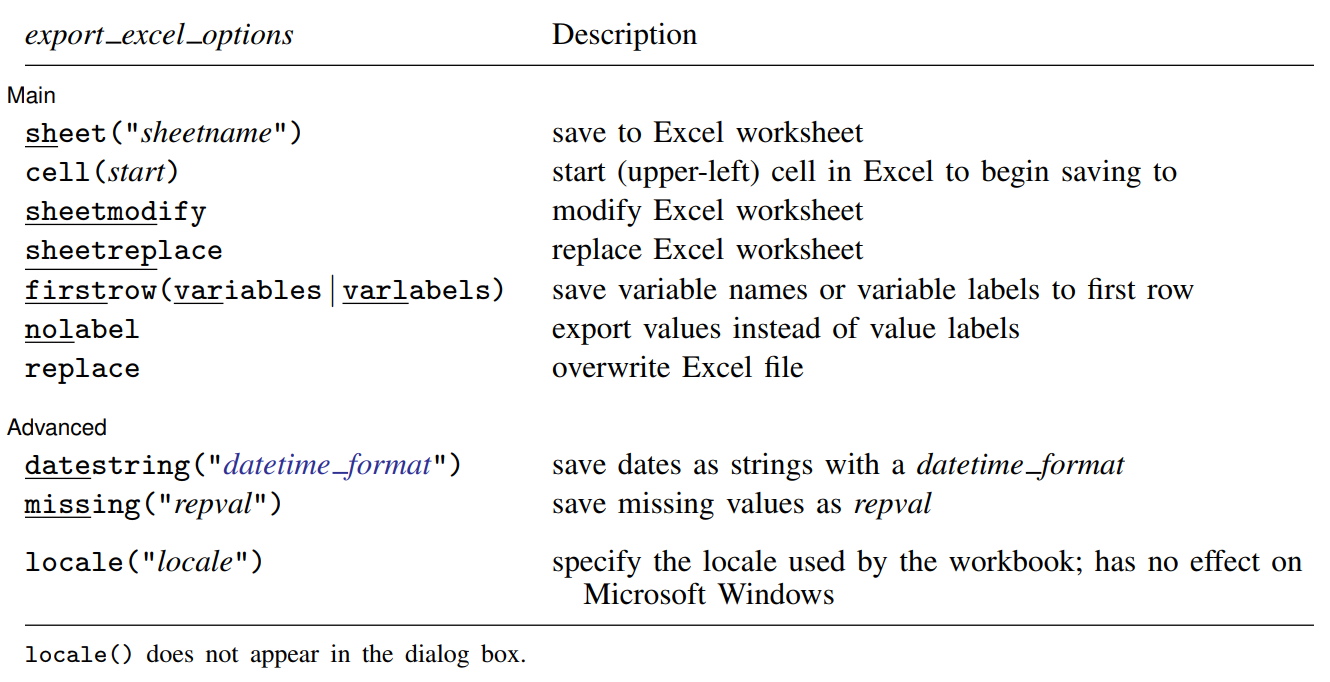
\includegraphics[width=\linewidth]{helpfile_exportexcel_2}
			\end{column}
		\end{columns}
	\end{frame}
	
	\begin{frame}
		\frametitle{\textsc{Task 9 - saving Stata datasets}}		
		\onslide<1-> Let's save the modified data as a dta file.
					\vspace{2mm} Type...
\begin{stlog}scatter m_used_ws m_drink_ws  || ///
lfit m_drink_ws m_used_ws
\end{stlog}
		\vspace{2mm}
		\onslide<2-> Notice that we use the \textbf{\textit{replace}} option. 
					 This overwrites the existing file. 
					 \vspace{2mm} Type the same command without \textbf{\textit{, replace}}, 
					 and see what error you get! 
		\vspace{2mm}			 
		\onslide<3-> Did you get an error like this? 
		\begin{center}			
			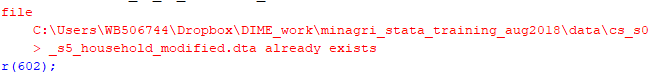
\includegraphics[width=0.8\linewidth]{error_save_existing}
		\end{center}
	\end{frame}
	
	\begin{frame}
		\frametitle{\textsc{Task 10 - exporting Stata datasets}}
			
		\onslide<1-> Now, let's save the modified data as a excel. 
					 This is helpful if you are sending the dataset to 
					 someone who does not use or have Stata. \\
					 Type...
		\vspace{2mm}
\begin{stlog}export excel using "$data\\cs_s0_s5_household_modified.xls", replace
\end{stlog}
		\vspace{2mm}
		\onslide<2-> Open the output file. 
					 Notice that it doesn't have variable names as column names.
					 This is very inconvenient!
		\onslide<3-> Use an optional command, \textbf{\textit{firstrow(variables)}}.
		\vspace{2mm}
\begin{stlog}export excel using "$data\\cs_s0_s5_household_modified.xls", /
> //
replace firstrow(variables)
\end{stlog}
		\vspace{2mm}
		\onslide <4-> Notice \textbf{///}. This is a way to let Stata now that multiple lines
					  constitute a single command. It's helpful when your command is getting too
					  long on your do file.
		\onslide<5-> Open the newly saved excel file. You will find column names!
	\end{frame}
		
	\section{Section 3: \\ Introduction to Stata Graphics}	
	
	\begin{frame}
	\frametitle{\textsc{Table gives all the details}}
		\begin{center}
		What's happening in this regression table? What's important?
		\begin{figure}
			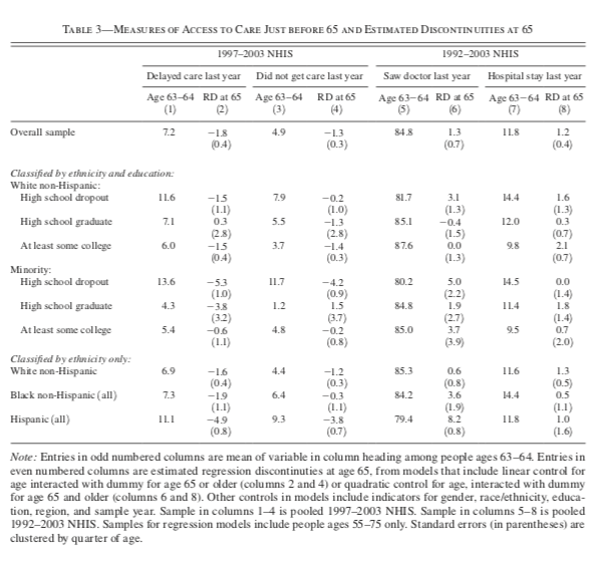
\includegraphics[width=0.7\linewidth]{reg_table_example}
		\end{figure}		
		\end{center}
	\end{frame}

	\begin{frame}
	\frametitle{\textsc{But figures \textit{tell the story}}}
		\begin{columns}
			\column{0.55\linewidth}
			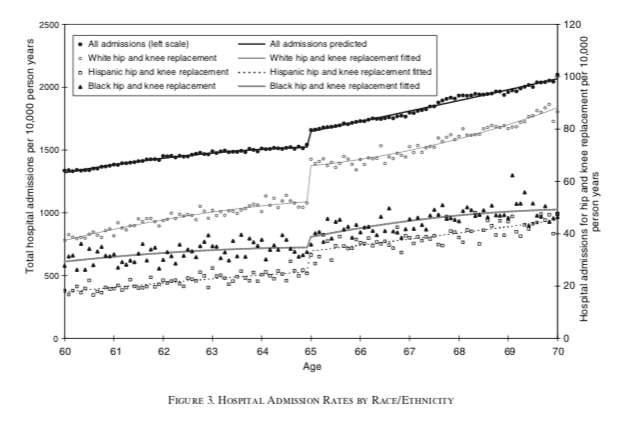
\includegraphics[height=5cm, width=6cm]{figure_example_1}
			\hspace{5mm}
			\column{0.45\linewidth}
			\begin{itemize}
				\item This is the data that generates those estimates.
				\item You can see exactly what is happening very quickly!
				\item Even more importantly: \\ \textbf{Your eyes are naturally drawn to the story!}
			\end{itemize}
		\end{columns} 
	\end{frame}

	\begin{frame}
	\frametitle{\textsc{Example: comparing means}}
		\begin{columns}
		\column{0.55\linewidth}
		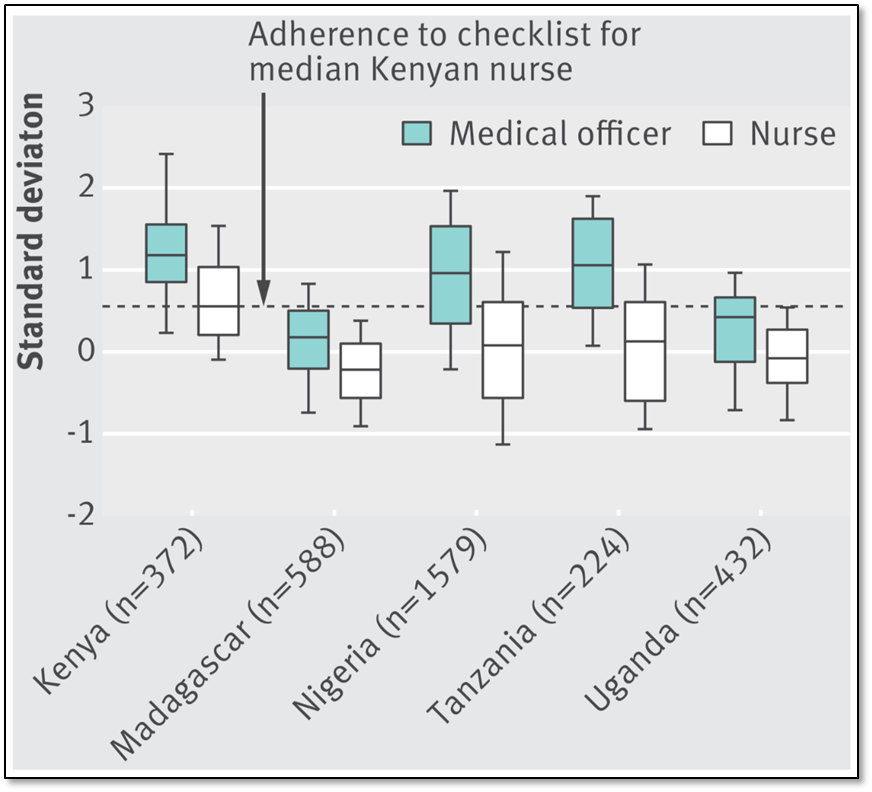
\includegraphics[height=5cm, width=6cm]{figure_example_2}
		\hspace{5mm}
		\column{0.45\linewidth}
		\begin{itemize}
			\item What is the main story in this graph? 
			\item We need more context to say something detailed about this, 
				  but what has the person creating the graph highlighted for us?
		\end{itemize}
		\end{columns} 
	\end{frame}
	
	
	\begin{frame}
	\frametitle{\textsc{Stata default graphs}}
		\begin{itemize}
			\item This is what a Stata graph looks like with very minimal 
				  customizing using optional commands
			\item Notice that there is no graph title. 
				  They are still informative, but need much improvement
			\item We will not go too deep to editing a Stata graph today,
				  but I'll show you have to make a graph and make some edits
				  for effective data visualization
		\end{itemize}	
		\begin{center}
			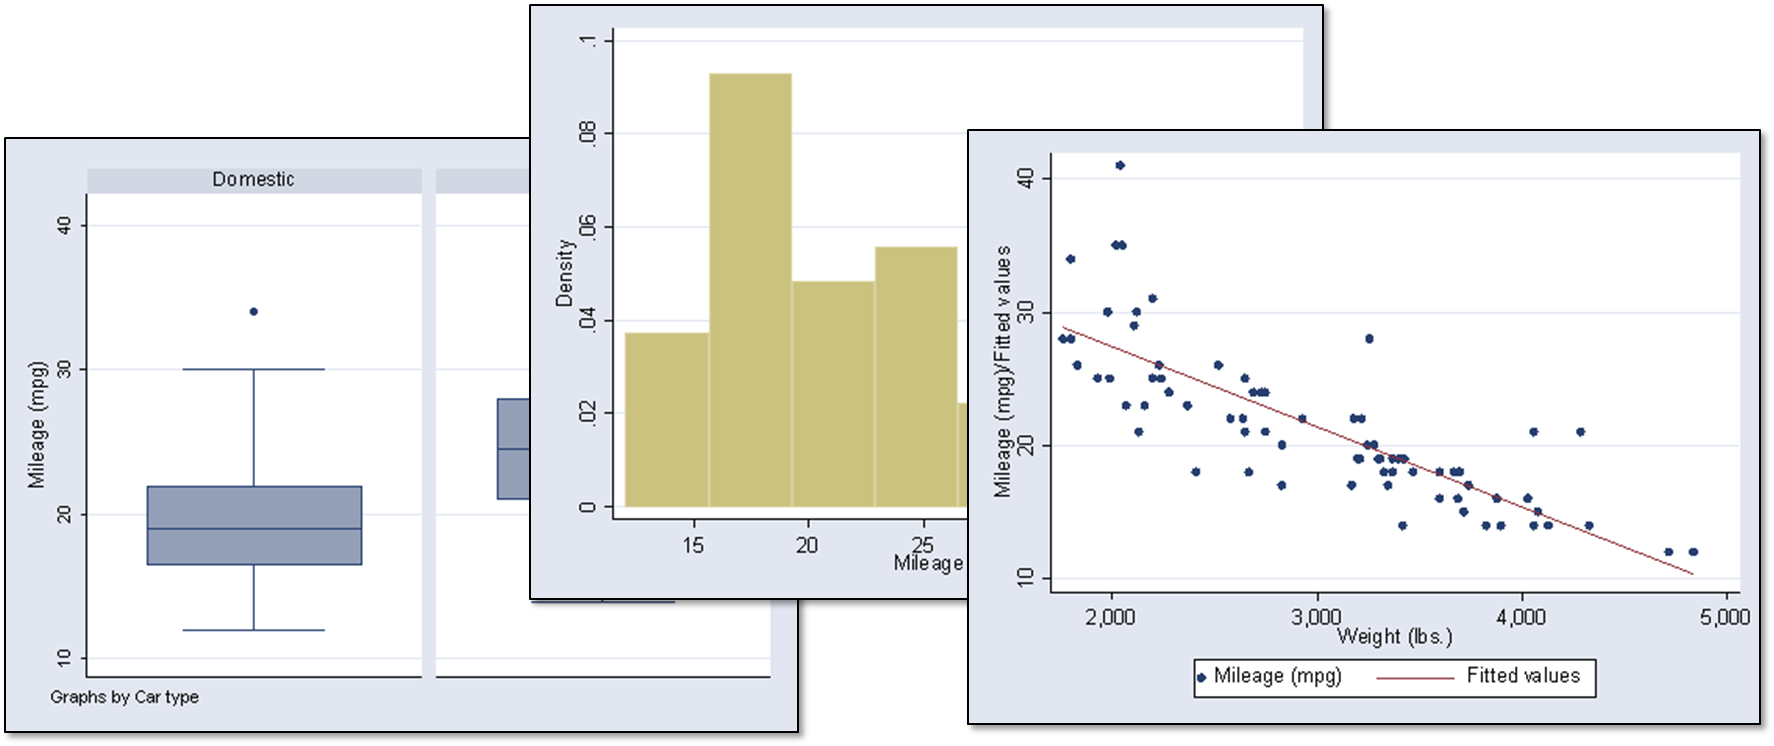
\includegraphics[width=\linewidth]{figure_example_3}
		\end{center}
	\end{frame}

	\begin{frame}
	\frametitle{\textsc{Stata has three core built-in graph functions.}}
		\begin{columns}
			\column{0.4\linewidth}
			\textbf{[graph \textit{graphtype}]} \\
			\small graphs which plot one or more variables on one axis \\ \vspace{2mm}
			\textbf{[twoway \textit{graphtype}]} \\
			\small graphs which plot two variables together on an x and y axis \\  \vspace{2mm}
			\small \textbf{\textit{twoway\_options}} is a set of optional commands that can be
					applied to all twoway graphs. \\
			\textbf{[histogram], [kdensity], [lowess]} \\
			\small Essential distributional commands
			\column{0.6\linewidth}
			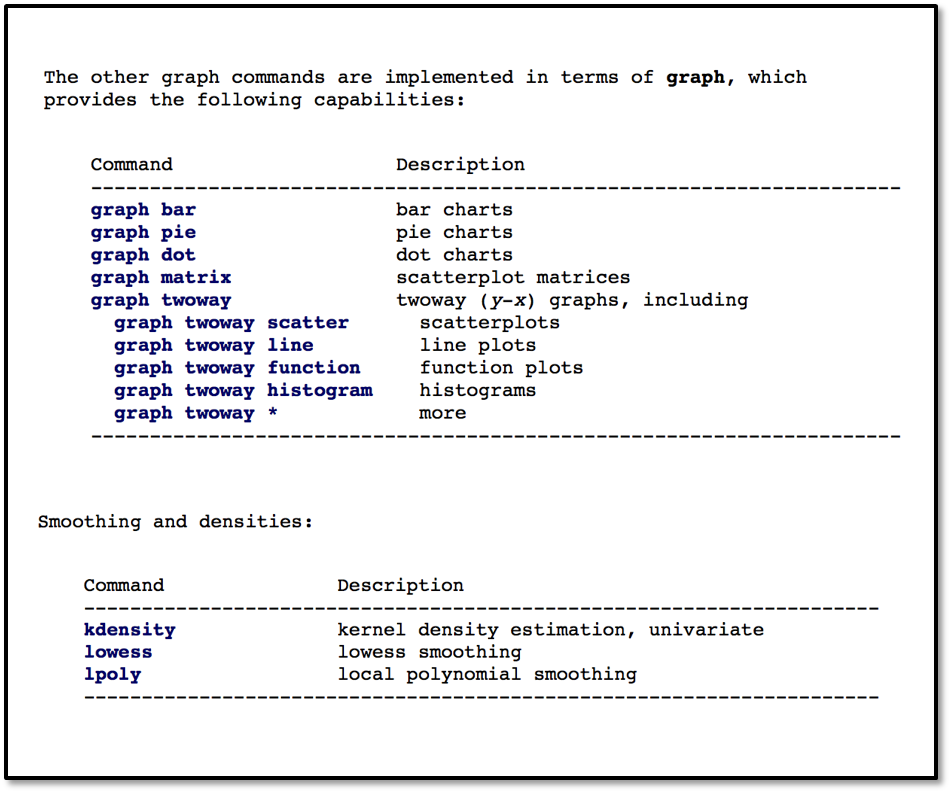
\includegraphics[height=6cm, width=7cm]{stata_builtin_graph_functions}
		\end{columns}
	\end{frame}
	
	\begin{frame}
	\frametitle{\textsc{Stata graph exercise 1}}
		\begin{center}
		\Large \textbf{Box plot}
		\end{center}
	\end{frame}	

	\begin{frame}
	\frametitle{\textsc{Box plot}}
		Let's make a a box plot like the one below using the variable, \textbf{m\_drink\_ws}.
		Notice a box plot is an example of a oneway graph. 
\begin{center}
    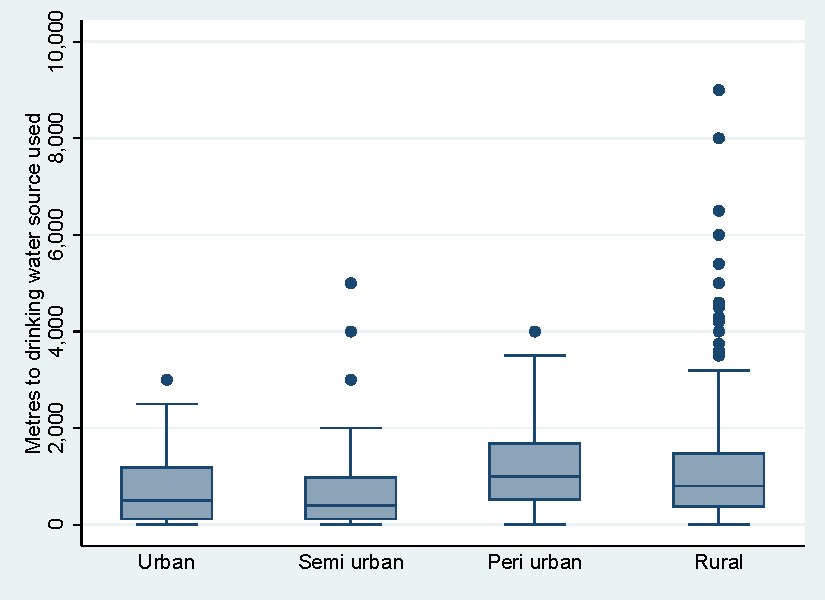
\includegraphics[width=0.8\textwidth]{boxplot_1.pdf}
\end{center}
	\end{frame}
	
	\begin{frame}
	\frametitle{\textsc{Box plot}}	
		\onslide<1-> Let's make a box plot from your do file.
		\begin{enumerate}
			 \item Open "\$data\_cs\_s0\_s5\_household\_modified.xls"
			 \item Type \textbf{\textit{search box plots}} in the command window to find out what command to be used.
					\textbf{\textit{search}} is a more general search through help files and other Stata resources.
			 \onslide<2-> \item The command should look like the following. Run from the do file.
		
\begin{stlog}graph box m_drink_ws
\end{stlog}
			\vspace{1mm}
			\onslide<3-> \item Notice the difference from earlier? 
			\vspace{1mm}			
		
\begin{center}
    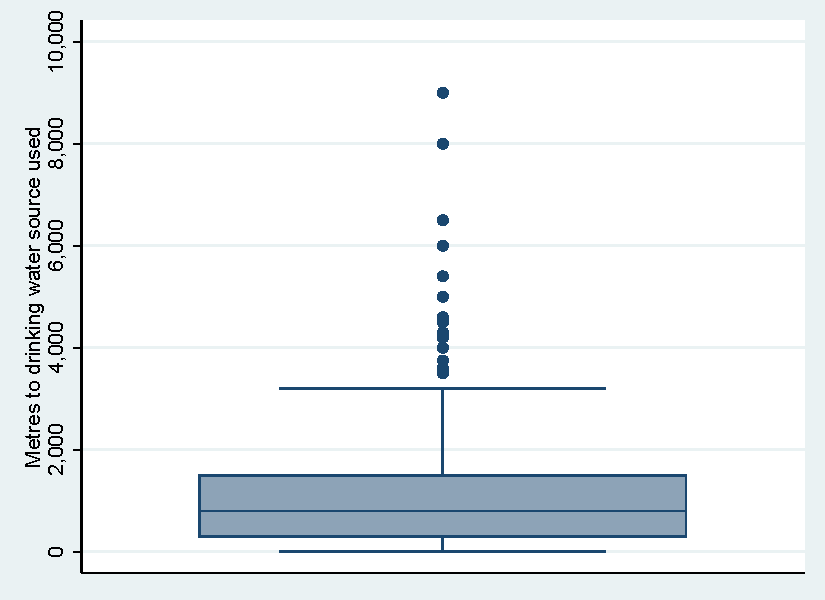
\includegraphics[width=0.5\textwidth]{boxplot_2.pdf}
\end{center}
		\end{enumerate}
	\end{frame}

	\begin{frame}
	\frametitle{\textsc{Box plot}}	
		\onslide<1-> Now, let's make multiple box plots by the residential environment, \textbf{urban\_2012}.
		\begin{enumerate}
			 \item Type \textbf{\textit{search box plots}} to see how to achieve this.
			 \onslide<2-> \item The optional commant, \textbf{\textit{over()}} can do this.
								Run the new \textbf{\textit{graph box}} command with the \textbf{\textit{over}} option.
		
\begin{stlog}graph box m_drink_ws, over(urban_2012)
\end{stlog}
\begin{center}
    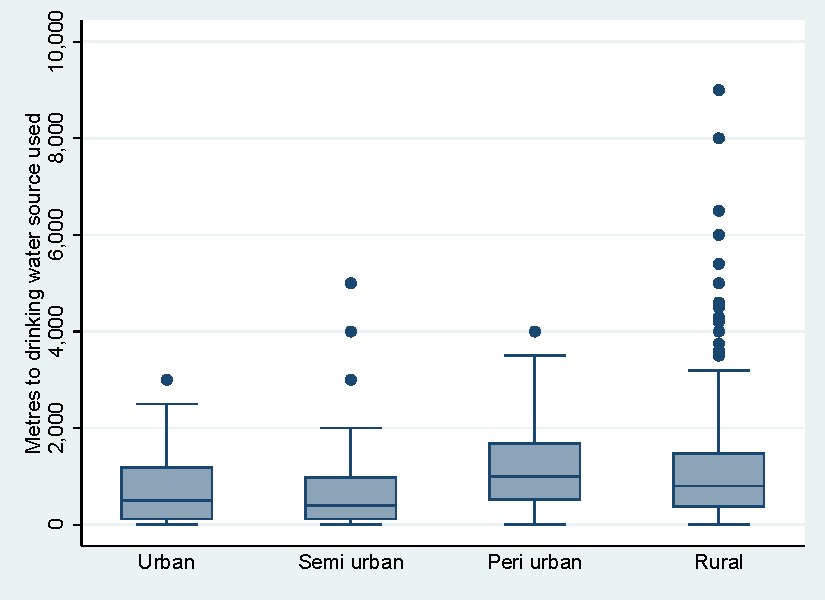
\includegraphics[width=0.5\textwidth]{boxplot_1.pdf}
\end{center}
		\end{enumerate}
	\end{frame}

	\begin{frame}
	\frametitle{\textsc{Stata graph exercise 2}}
		\begin{center}
		\Large \textbf{Histogram}
		\end{center}
	\end{frame}		
	
	\begin{frame}
	\frametitle{\textsc{Histogram}}
		Let's make a histogram like the one below using the variable, \textbf{m\_drink\_ws}.
		Notice that a histogram is an example of a twoway graph.
	
\begin{center}
    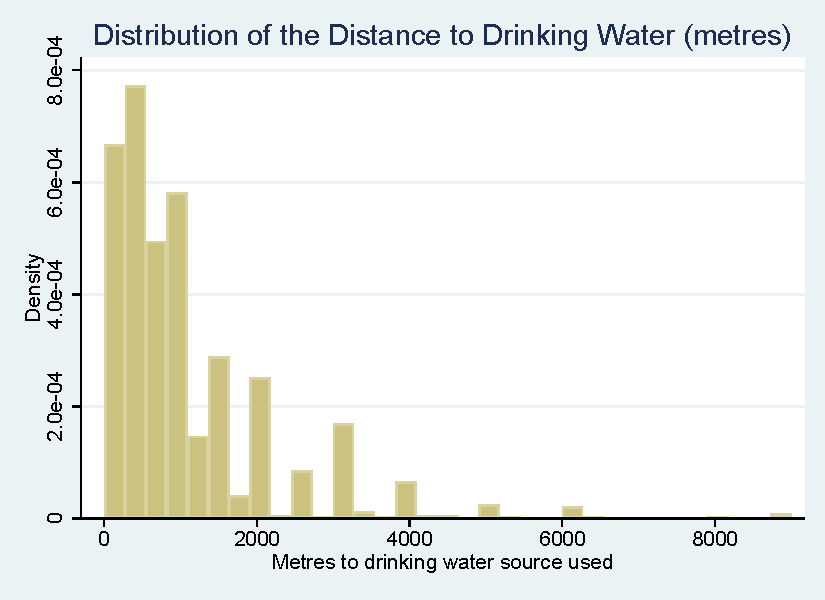
\includegraphics[width=0.8\textwidth]{hist_1.pdf}
\end{center}
	\end{frame}
	
	\begin{frame}
	\frametitle{\textsc{Histogram}}	
		\onslide<1-> Let's make a histogram from your do file.
		\begin{enumerate}
			 \item Type \textbf{\textit{help histogram}} in the command window to find out what command to be used.
			 \onslide<2-> \item The command should look like the following. Run from the do file.
		
\begin{stlog}. tabstat m_main_ws m_used_ws
{\smallskip}
   stats {\VBAR}  m_main{\tytilde}s  m_used{\tytilde}s
\HLI{9}{\PLUS}\HLI{20}
    mean {\VBAR}  791.2462   863.863
\HLI{9}{\BOTT}\HLI{20}
{\smallskip}
\end{stlog}
			\vspace{2mm}
			\onslide<3-> \item Notice the difference from earlier? We need the title.
			\vspace{2mm}
		
\begin{center}
    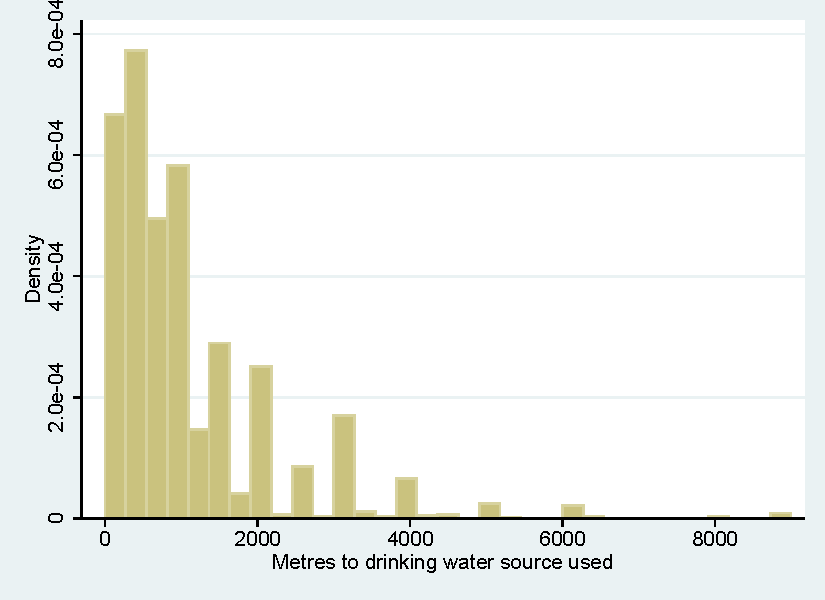
\includegraphics[width=0.5\textwidth]{hist_2.pdf}
\end{center}
		\end{enumerate}
	\end{frame}

	\begin{frame}
	\frametitle{\textsc{Histogram}}	
		\onslide<1-> Now, let's add the title. You can also choose your own title that is informative.
					 Notice in general a good title is informative but short.
		\begin{enumerate}
			 \onslide<2-> \item The optional command, \textbf{\textit{title()}} can do this.
								Run the new \textbf{\textit{histogram}} command with 
								the \textbf{\textit{title}} option.
		
\begin{stlog}histogram m_drink_ws, ///
title("Distribution of the Distance to Drinking Wat
> er (metres)")
\end{stlog}
			\vspace{1mm}
			\onslide <4-> \item \textbf{\textit{help twoway\_options}} to find out more about the \textbf{\textit{title}} option and more.
		\end{enumerate}
	\end{frame}
	
	\begin{frame}
		\frametitle{\textsc{Refresher}}
		Yesterday we learnt ...
		\begin{itemize}
			\item how to use do-files
			\item how to write comments in do-files
			\item how to save and export datasets
			\item how to create simple graphs
		\end{itemize}
	\end{frame}
	
	\begin{frame}
	\frametitle{\textsc{Histogram}}
		\onslide<1-> I wanted to start today by adding onto the histrogram we made yesterday.
		\onslide<2-> The optional command, \textbf{\textit{by()}} 
					 splits by a categorical variable. Try:
	
\begin{stlog}import excel using "$data\\cs_s0_s5_household_modifi
> ed.xls", ///
clear firstrow
\end{stlog}
		\onslide<3-> Does your graph look like this?
	
\begin{center}
    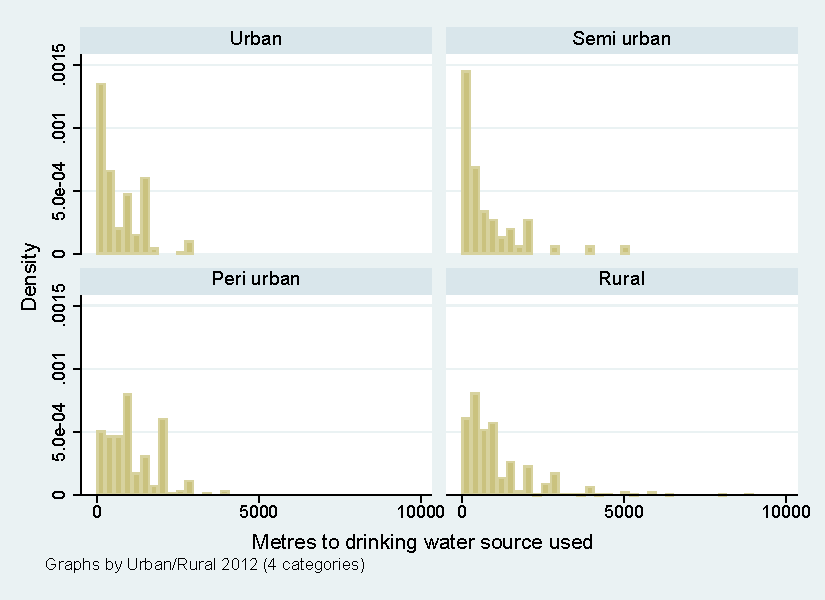
\includegraphics[width=0.8\textwidth]{hist_3.pdf}
\end{center}
	\end{frame}
	

	\begin{frame}
	\frametitle{\textsc{Stata graph exercise 3}}
		\begin{center}
		\Large \textbf{Bar graph}
		\end{center}
	\end{frame}		
	
	\begin{frame}
	\frametitle{\textsc{Bar graph}}
		Let's make a bar graph like the one below using the variable, \textbf{d\_closest\_ws} and \textbf{urban\_2012}.
		\vspace{1mm}
	
\begin{center}
    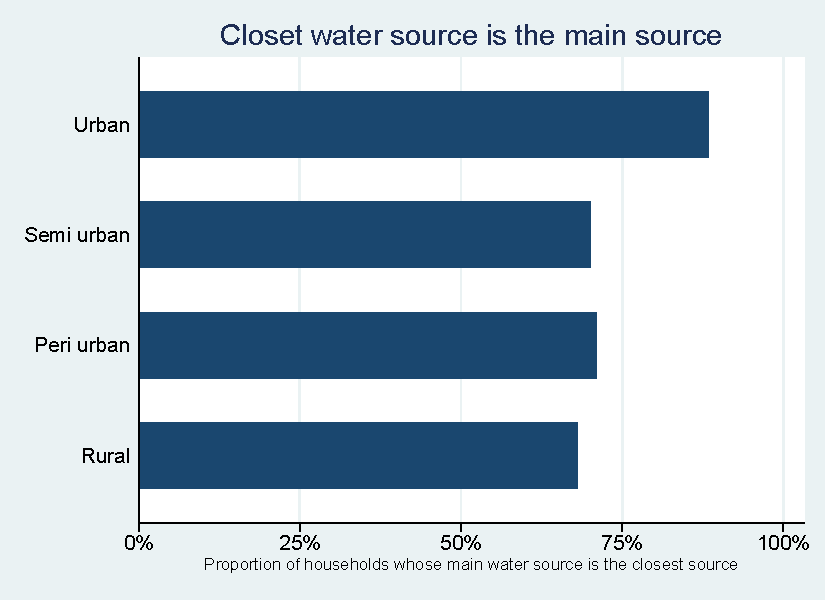
\includegraphics[width=0.8\textwidth]{bar_1.pdf}
\end{center}
	\end{frame}
	
	\begin{frame}
	\frametitle{\textsc{Bar graph}}	
		\onslide<1-> Let's make a bar graph from your do file.
		\begin{enumerate}
			 \item Type \textbf{\textit{help graph bar}} in the command window 
				   to find out what command to be used.
			 \onslide<2-> \item Note that you can make vertical or horizontal 
								bars with this commands. The basic command should
								look like this.
		
\begin{stlog}scatter m_used_ws m_drink_ws  || ///
lfit m_drink_ws m_used_ws
\end{stlog}
			\vspace{1mm}
			\onslide<3-> \item Recall the \textbf{\textit{over}} option.
			\vspace{1mm}
			\onslide<4-> \item It should look something like this.
		
\begin{stlog}scatter m_used_ws m_drink_ws  || ///
lfit m_drink_ws m_used_ws, ///
        ytitle("Distance to the nearest drinking water source") ///
        xtitle("Distance to the main drinking source used") ///
        title("Is the main drinking water also the closest source?")
\end{stlog}
		\end{enumerate}
	\end{frame}
	
	\begin{frame}
	\frametitle{\textsc{Bar graph}}	
		\onslide<1-> Now we need to add the main and y axis titles.
					 Recall yesterday's lesson and try on your own. \vspace{1mm}
		\onslide<2-> Does your command and graph look like this?
		
\begin{center}
    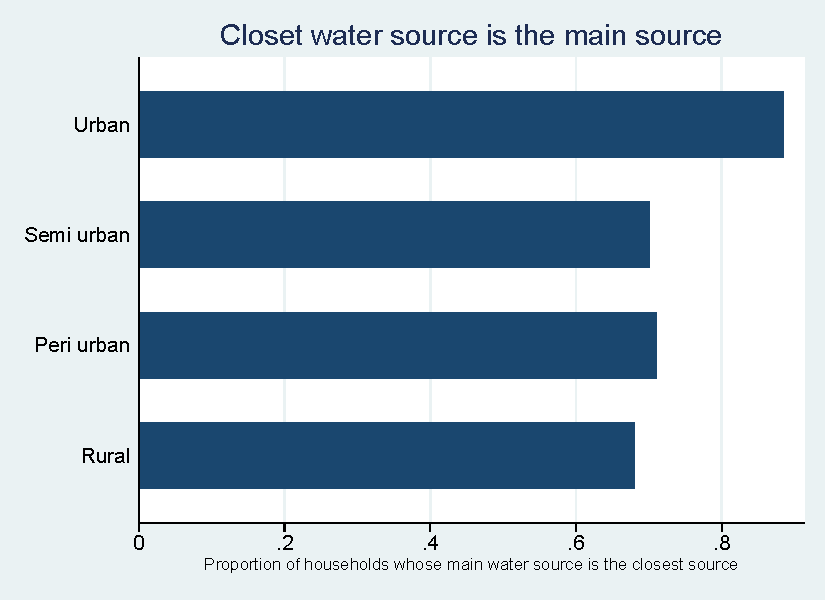
\includegraphics[width=0.8\textwidth]{bar_2.pdf}
\end{center}
			\vspace{1mm}
		\onslide<3-> Something is still missing...
	\end{frame}

	\begin{frame}
	\frametitle{\textsc{Bar graph}}	
		\onslide<1-> The y axis has unintuitive labels. This is proportion.
					 So let's convert to percentage. We can achieve this with 
					 the optional command, \textbf{\textit{ylabel}}. \vspace{1mm}
	
\begin{stlog}graph hbar d_closest_ws , over(urban_2012) ///
        title("Closet water source is the main source") ///
        ylabel(0 "0\%" .25 "25\%" .5 "50\%" .75 "75\%" 1 "100\%") ///
        ytitle("Proportion of households whose main water source is the closest source", size(small))
\end{stlog}
	\end{frame}
	
	\begin{frame}
	\frametitle{\textsc{Stata graph exercise 4}}
		\begin{center}
		\Large \textbf{Scatter plot}
		\end{center}
	\end{frame}		
	
	\begin{frame}
	\frametitle{\textsc{Scatter plot}}
		Let's make a scatter plot with a fitted line like the one below using the variable, \textbf{m\_drink\_ws} and \textbf{m\_used\_ws}.
		Notice that a scatter plot with a fitted line is an example of a twoway graph.
		\vspace{1mm}
	
\begin{center}
    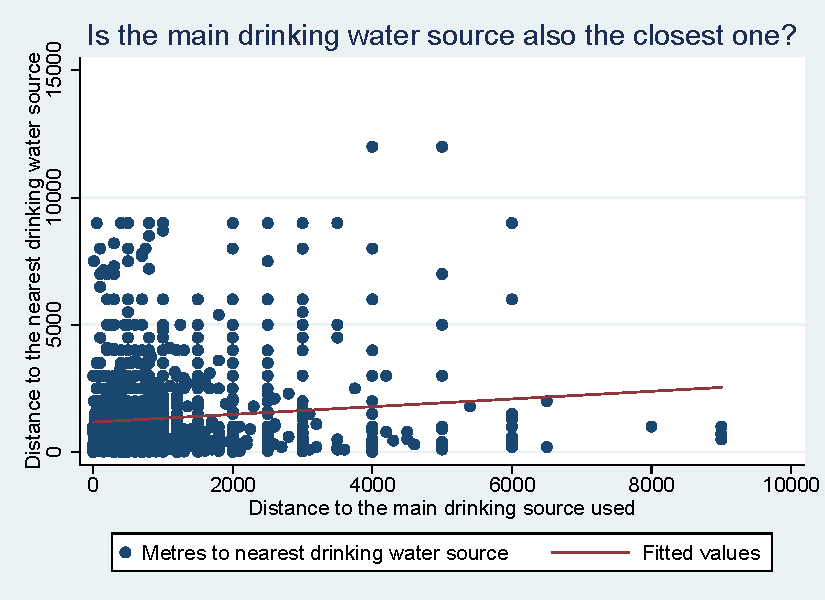
\includegraphics[width=0.8\textwidth]{scatter_1.pdf}
\end{center}
	\end{frame}
	
	\begin{frame}
	\frametitle{\textsc{Scatter plot}}	
		\onslide<1-> Let's make a scatter plot from your do file.
		\begin{enumerate}
			 \item Type \textbf{\textit{help scatter}} in the command window to find out what command to be used.
			 \onslide<2-> \item The command should look like the following. Run from the do file.
		
\begin{stlog}The result is 12.
{\smallskip}
\end{stlog}
			\vspace{1mm}
			\onslide<3-> \item Notice the difference from earlier? No fitted line!
			\vspace{1mm}
		
\begin{center}
    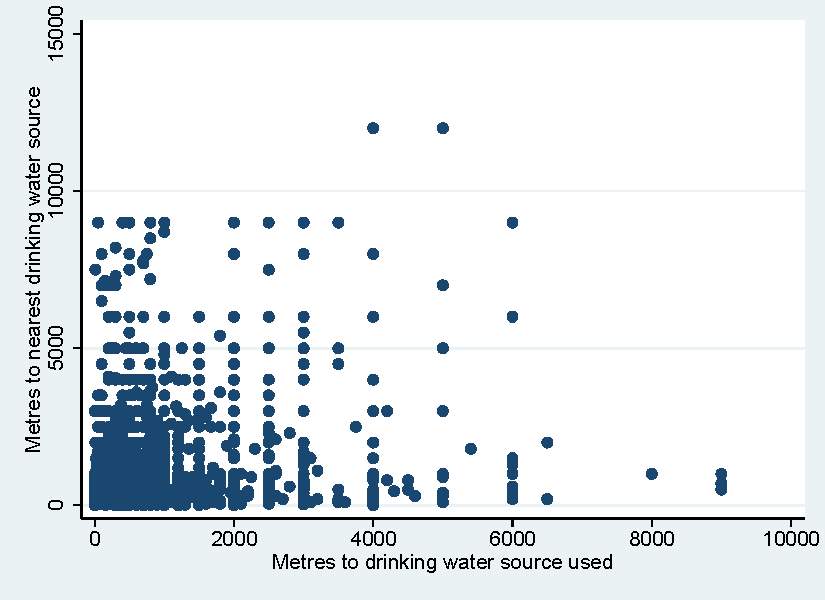
\includegraphics[width=0.5\textwidth]{scatter_2.pdf}
\end{center}
		\end{enumerate}
	\end{frame}
	
	\begin{frame}
	\frametitle{\textsc{Scatter plot}}	
		\onslide<1-> Let's add a fitted line. Type \textbf{\textit{help lfit}} to learn how to do this.
		\begin{enumerate}
			 \onslide<2-> \item You may notice that this is an entirely different command. 
								Stata can actually overlay multiple twoway graphs. 
								To do this, run the following command.
								Notice that \textbf{$\Vert$} is a way to overlay the graphs.
		
\begin{stlog}destring earnings_sell_w, replace
\end{stlog}
			\vspace{1mm}
			\onslide<3-> \item Notice the difference from earlier? No main title and y and y titles!
			\vspace{1mm}
		
\begin{center}
    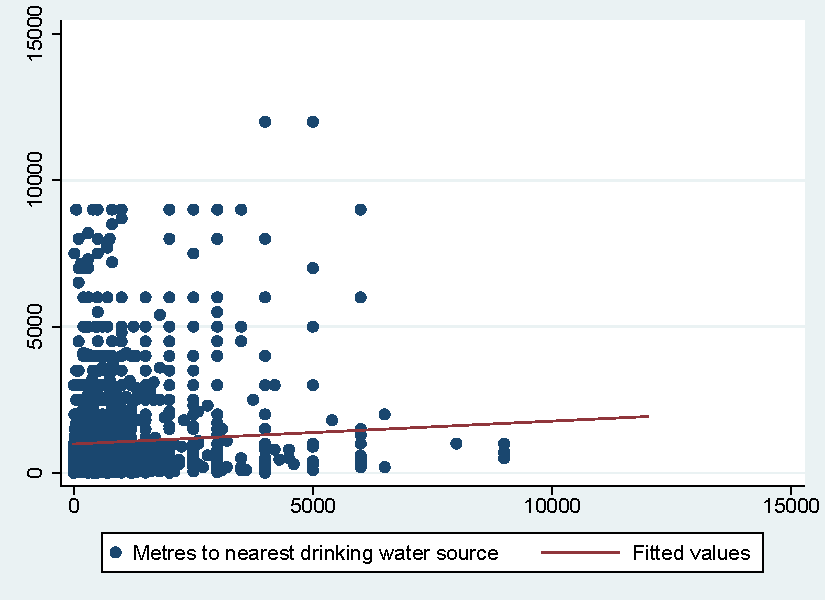
\includegraphics[width=0.5\textwidth]{scatter_3.pdf}
\end{center}
		\end{enumerate}
	\end{frame}

	\begin{frame}
	\frametitle{\textsc{Scatter plot}}	
		\onslide<1-> This is because the fitted line is a linear prediction and 
					 no longer represents the raw distance values. 
					 But we can simply add on titles that can be helpful for the graph's intended audience.
		\begin{enumerate}
			 \onslide<2-> \item Recall the \textbf{\textit{twoway\_options}}, and the \textbf{\textit{title()}} option.
								You can use the same option and very similar options called \textbf{\textit{xtitle()}} and
								\textbf{\textit{ytitle()}}.
		
\begin{stlog}scatter m_used_ws m_drink_ws  || ///
<<<<<<< HEAD
lfit m_used_ws m_drink_ws, ///
        ytitle("Distance to the nearest drinking water source
> ") ///
        xtitle("Distance to the main drinking source used") /
> //
        title("Is the main drinking water also the closest so
> urce?")
=======
lfit m_drink_ws m_used_ws, ///
        ytitle("Distance to the nearest drinking water source") ///
        xtitle("Distance to the main drinking source used") ///
        title("Is the main drinking water also the closest source?")
>>>>>>> master
\end{stlog}
		\end{enumerate}
	\end{frame}
	
	\begin{frame}
	\frametitle{\textsc{Stata graph exercise 3}}
		\begin{center}
		\Large \textbf{Saving and combining graphs}
		\end{center}
	\end{frame}	
	
	\begin{frame}
	\frametitle{\textsc{Saving a Stata graph}}
		Let's save all 3 graphs we made today.
		\begin{enumerate}
			\item To do so, add \textbf{\textit{graph save}} after each of your graphs like the following.
	
			\item Notice that you need to specify where you want save it,
				  and how you want to name it.
		\end{enumerate}
	\end{frame}
	
	\begin{frame}
	\frametitle{\textsc{Combining Stata graphs}}
		Let's combine all 3 graphs we made today.
		\begin{enumerate}
			\item To do so, add \textbf{\textit{graph combine}} after each of your graphs like the following.
	
			\item Notice that you need to specify where you want save it,
				  and how you want to name it.
		\end{enumerate}
	\end{frame}
	
	\begin{frame}
	\frametitle{\textsc{Combining Stata graphs}}
		\onslide<1-> Does yours look like this?
	
\begin{center}
    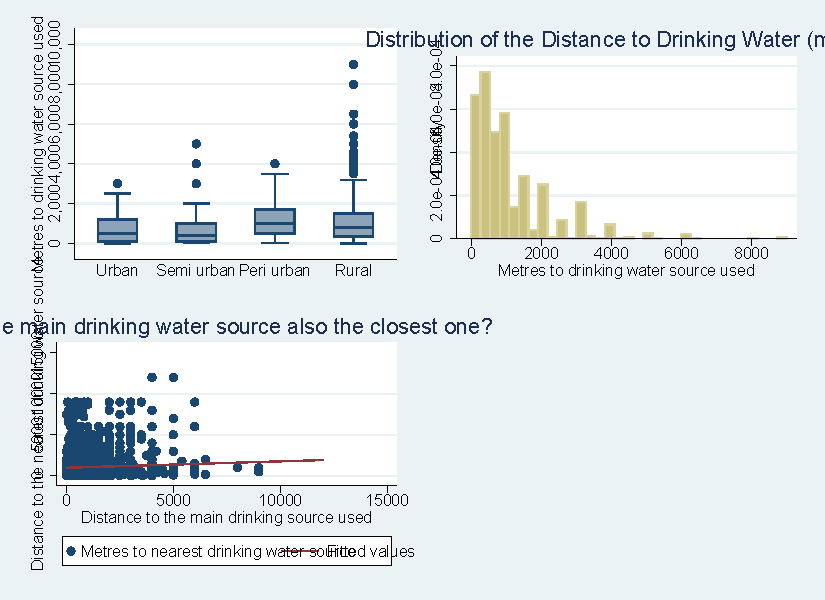
\includegraphics[width=0.5\textwidth]{combined.pdf}
\end{center}
		\begin{itemize}
			\onslide<2-> \item Why look so ugly?
			\onslide<3-> \item Luckily, there are ways to make this nice like this.			
		\end{itemize}
	\end{frame}
				
	\begin{frame}
	\frametitle{\textsc{Combining Stata graphs}}
		There are many ways to make it look better like the following. \\
		The solution do file will contain the commands to make the below graph. \\
		Change it around and have fun with it! \\
		Remember help files are your best friend.
	
\begin{center}
    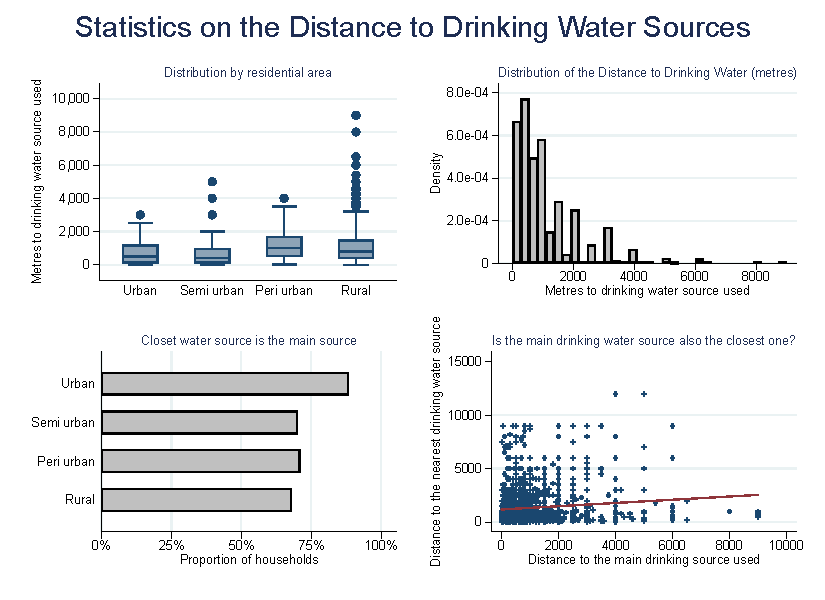
\includegraphics[width=0.5\textwidth]{combined_better.pdf}
\end{center}
	\end{frame}
	
	\begin{frame}
		\frametitle{\textsc{Importing an excel file}}
		\begin{itemize}
		\item You can import an excel using the drop down menus:
		File $\rightarrow$ Import $\rightarrow$ Excel spreadsheet
		\item You can also write a command to import an excel file
		\item Let us import the excel file we saved yesterday
		\end{itemize}
		
\begin{stlog}import excel using "$data\\cs_s0_s5_household_modified.xls", /
> //
clear firstrow
\end{stlog}
		
		
		
	\end{frame}
	
	\begin{frame}
		\frametitle{\textsc{Destringing}}

		\begin{itemize}
			\item Sometimes numbers are be stored as text
			\item We can convert numbers stored as strings to numbers by using the \textit{destring} command
			\item Let us try converting the variable \textit{earnings\_sell\_w} to a numeric variable
		\end{itemize}
\begin{stlog}destring earnings_sell_w, replace
\end{stlog}
	\end{frame}
		\begin{frame}
	\frametitle{\textsc{Some Stata do's and don't}}
	\begin{itemize}
		  \item NEVER save over the existing dataset (especially a raw dataset)!
		  \item Comment on why, not on what
		
		\item Always write a do-file
		  \item Make sure your work flow works smoothly
		  \item Provide concise and self explanatory titles to graphs
	  \end{itemize}
	 \end{frame}	
	 
	 
	 
	\section{Extra section: More about Stata}
	


	\begin{frame}
	\frametitle{\textsc{Missing values}}
		\begin{itemize}
			\item String variables can be empty, but numeric variables can't be empty. 
				  Instead numeric variables have something called “missing values”.
				\begin{itemize}
					\item Missing values are represented in Stata with a period as in " \textbf{.} ". 
					\item You can also use .a or .b etc. to .z for missing values 
						  and you will learn later how these can be used
				\end{itemize}
			\item Stata can't use missing values in computations (averages, regressions etc.) 
				  so it skips observations with missing values . 
			\item Missing values changes the analysis as observations with 
				  missing values are excluded from commands like summarize and regress.
			\item Good practice to always check for missing values when tabulating variables.			
		\end{itemize}
	\end{frame}
	
	
	\begin{frame}
		\frametitle{\textsc{Using drop down menus to create graphs}}
		
		\begin{itemize}
			\item It is hard to remember all the commands and options in general and especially to create graphs
			\item We can use drop down menus to create the graph
			\item For instance, if we want to create a pie chart for the variable \textit{urban\_2012} using dropdown menus we can follow these steps
			\end{itemize}
			Graphics $\rightarrow$ Pie chart, select \textit{urban\_2012} as Category variable and press OK
		
	\end{frame}
	
	

	\begin{frame}
	\frametitle{\textsc{Macros - locals}}
		\begin{center}
			\onslide<1-> \LARGE \textbf{Defining macros - local}
		\end{center}
		Type in your dofile the following and \textit{run all the lines at once}.
		\begin{itemize}
			\item Note that \textbf{`} is not the same as \textbf{'}.
\begin{stlog}histogram m_drink_ws, ///
fcolor(gs12) lcolor(black) lwidth(medium) ///
title("Distribution of the Distance to Drinking Water (metres)", ///
          size(small)) ///
xtitle(, size(small)) ///                               
ytitle(, size(small)) ///                               
ylabel(, angle(0) labsize(small)) ///
xlabel(, labsize(small)) ///
graphregion(color(white))                               
\end{stlog}
		\vspace{2mm}
		\onslide<2-> \item What did the result say?
		\onslide<3-> 
\begin{stlog}graph hbar d_closest_ws , ///
over(urban_2012, label(labsize(small))) ///
bar(1, fcolor(gs12) lcolor(black) lwidth(medium)) ///
title("Closet water source is the main source", ///
          size(small)) ///      
ylabel(0 "0\%" .25 "25\%" .5 "50\%" .75 "75\%" 1 "100\%", ///
          labsize(small)) ///
ytitle("Proportion of households", size(small)) ///
graphregion(color(white))                               
\end{stlog}
			\onslide<4-> \item Try running them one by one, and see what happens?
				\begin{itemize}
					\onslide<5-> \item It probably didn't run. 
									   This is one of the major differences between global and local.
									   Local is really local and only last within a single run.
									   For more please refer to the help file on \textit{macro}.
				\end{itemize}
		\end{itemize}
	\end{frame} 
	


		
	\begin{frame}
	\frametitle{\textsc{tabstat}}
		\begin{itemize}
			\item While \textbf{\textit{summarize}} and \textbf{\textit{tabulate}} 
				  provide useful fixed format output, 
				  \textbf{\textit{tabstat}} gives you the ability specify 
				  exactly what statistics you want in your input.
			\item By default, \textbf{\textit{tabstat}} only disply the mean.
			\item We can add a whole range of statistics using the option 
				  \textbf{\textit{statistics()}}. 
				  See \textbf{\textit{help tabstat}}, for a list of the statistics you can add.
		\end{itemize}
	\end{frame}
	
	\begin{frame}
	\frametitle{\textsc{tabstat}}
		Here are some examples.
		\begin{itemize}
			\item This is the very basic command.
\begin{stlog}scatter m_used_ws m_drink_ws, ///
        msize(small) msymbol(plus) || ///
lfit m_used_ws m_drink_ws, ///
        ylabel(, angle(0) labsize(small)) ///
legend(off) ///
xlabel(, labsize(small)) ///
ytitle("Distance to the nearest drinking water source", ///
           size(small)) ///
xtitle("Distance to the main drinking source used", ///
           size(small)) ///
title("Is the main drinking water source also the closest one?", ///
          size(small)) ///
graphregion(color(white))                                                       
\end{stlog}
			\vspace{2mm}
			\item You can add multiple variable at a time.
\begin{stlog}graph combine ///
        "$script/box_better.gph" ///
        "$script/histogram_better.gph" ///      
        "$script/bar_better.gph" ///                         
>            
        "$script/scatter_better.gph", ///
        graphregion(color(white)) ///
        title("Statistics on the Distance to Drinking Water S
> ources")
\end{stlog}
		\end{itemize}
	\end{frame}
		
	\begin{frame}
	\frametitle{\textsc{tatstat}}
	Lastly...
		\begin{itemize}
			\vspace{2mm}
			\item You choose what types of statistics you want it to display.
\begin{stlog}import excel using "$data\\cs_s0_s5_household_modified.xls", /
> //
clear firstrow
\end{stlog}
		\end{itemize}
	\end{frame}
	
	\begin{frame}
	\frametitle{DIME Resources}
		\begin{center}
		\begin{columns}
		\column{0.4\linewidth}
		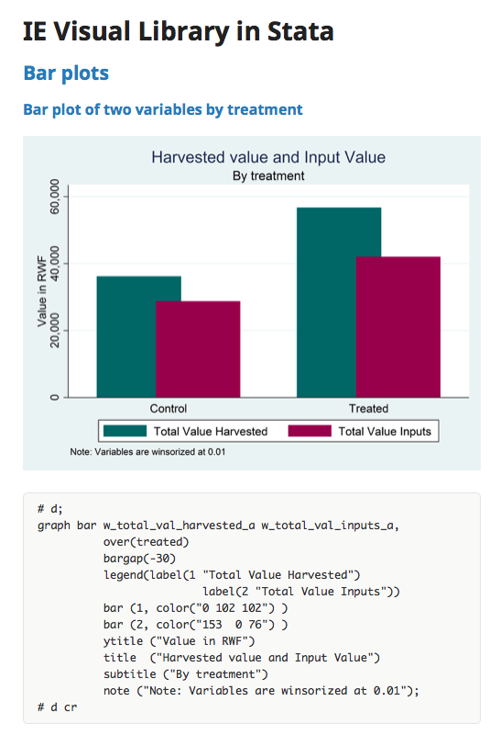
\includegraphics[height=5cm, width=3.5cm]{dime_resource_1} \\
		\tiny \url{https://worldbank.github.io/Stata-IE-Visual-Library/}
		\column{0.6\linewidth}
		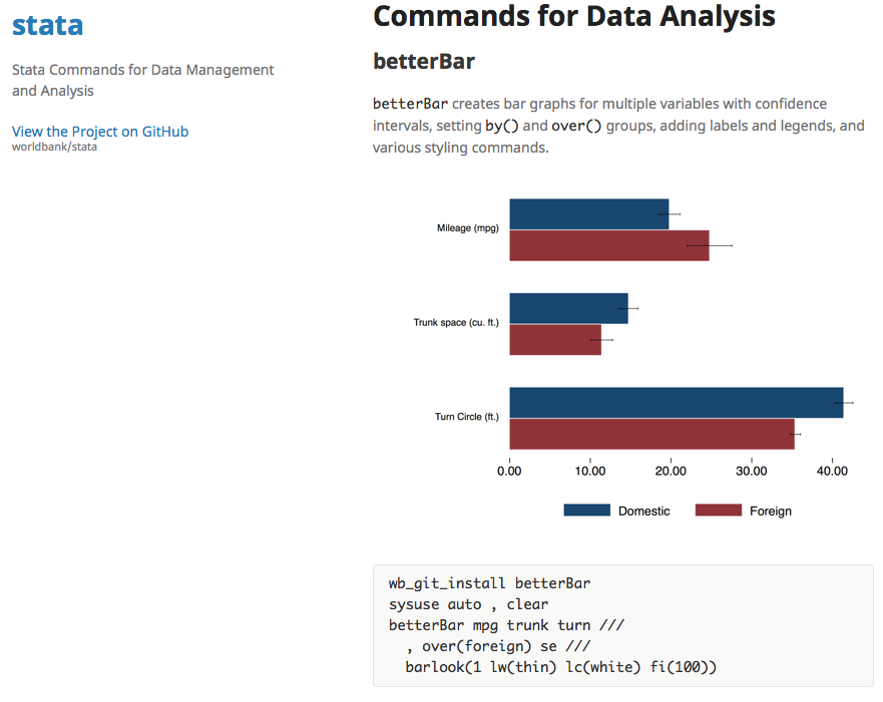
\includegraphics[height=5cm, width=6cm]{dime_resource_2} \\
		\tiny \url{https://worldbank.github.io/stata/}
		\end{columns}	
		\end{center}
	\end{frame}
	
	\begin{frame}
		\begin{center}
			\Large Murakoze neza! \\
			\vspace{10mm}
			\normalsize Sakina Shibuya and Roshni Khincha \\
			\small (\url{sshibuya@worldbank.org})
			\small (\url{rkhincha@worldbank.org})		
		\end{center}
	\end{frame}	
	
	\end{document}
